\clearpage

\section{Comparison of \RunPeriod to \PrevRunPeriod for Asimov A sensitivities}
\label{app:asimov_comparison}

This chapter compares the expected Asimov A sensitivities for the current \RunPeriod to those of the previous \PrevRunPeriod period.

\subsection{Results for \appearance}
In \cref{fig:ssqth13_vs_dcp_asimov_compare} the result for \appearance with reactor constraint and T2K only is shown.

\begin{figure*}[htb]
	\center
	\begin{subfigure}[b]{0.49\textwidth}
		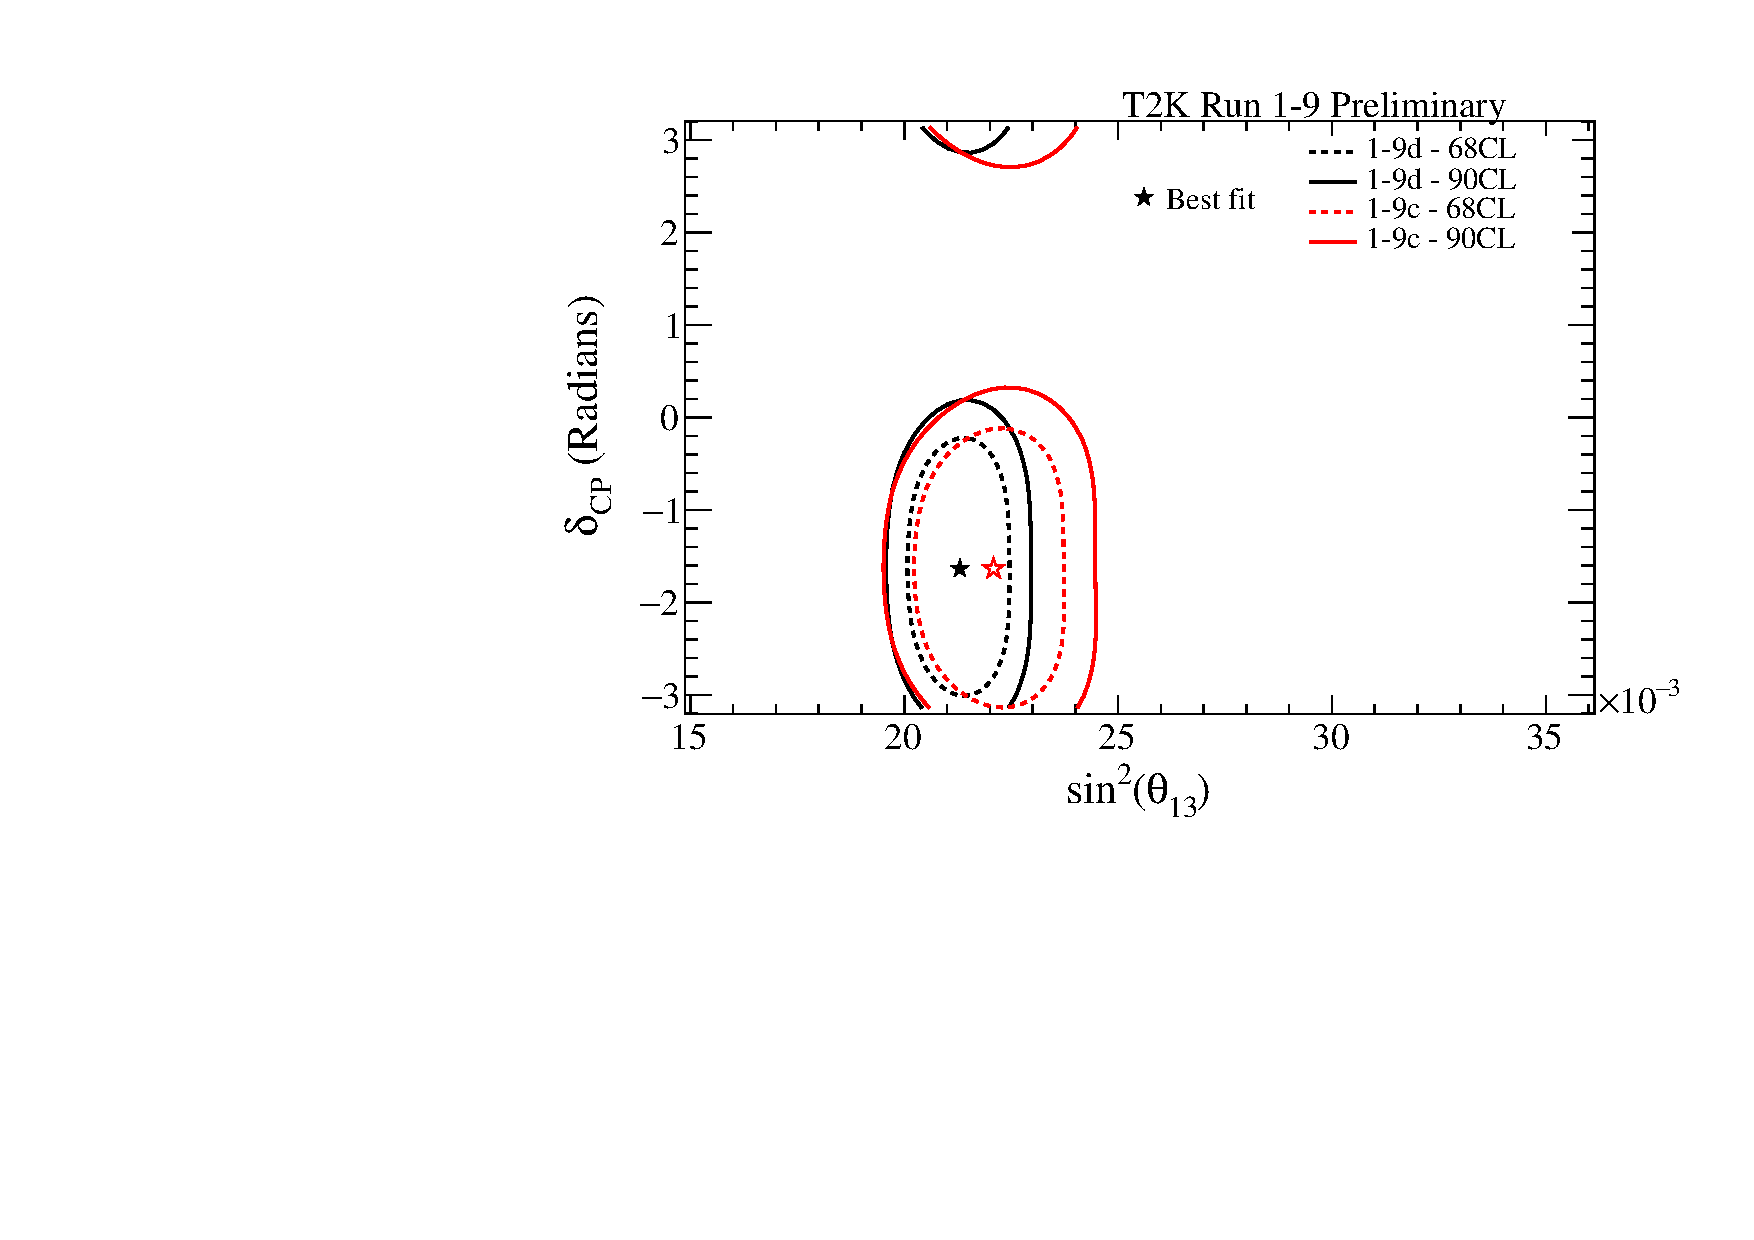
\includegraphics[width=0.9\textwidth]{images/sensitivity/comparison/appearance_wrc_normal_1-9d_v_1-9c}
		\caption{\appearance NH with reactor constraint}
	\end{subfigure}
	\begin{subfigure}[b]{0.49\textwidth}
		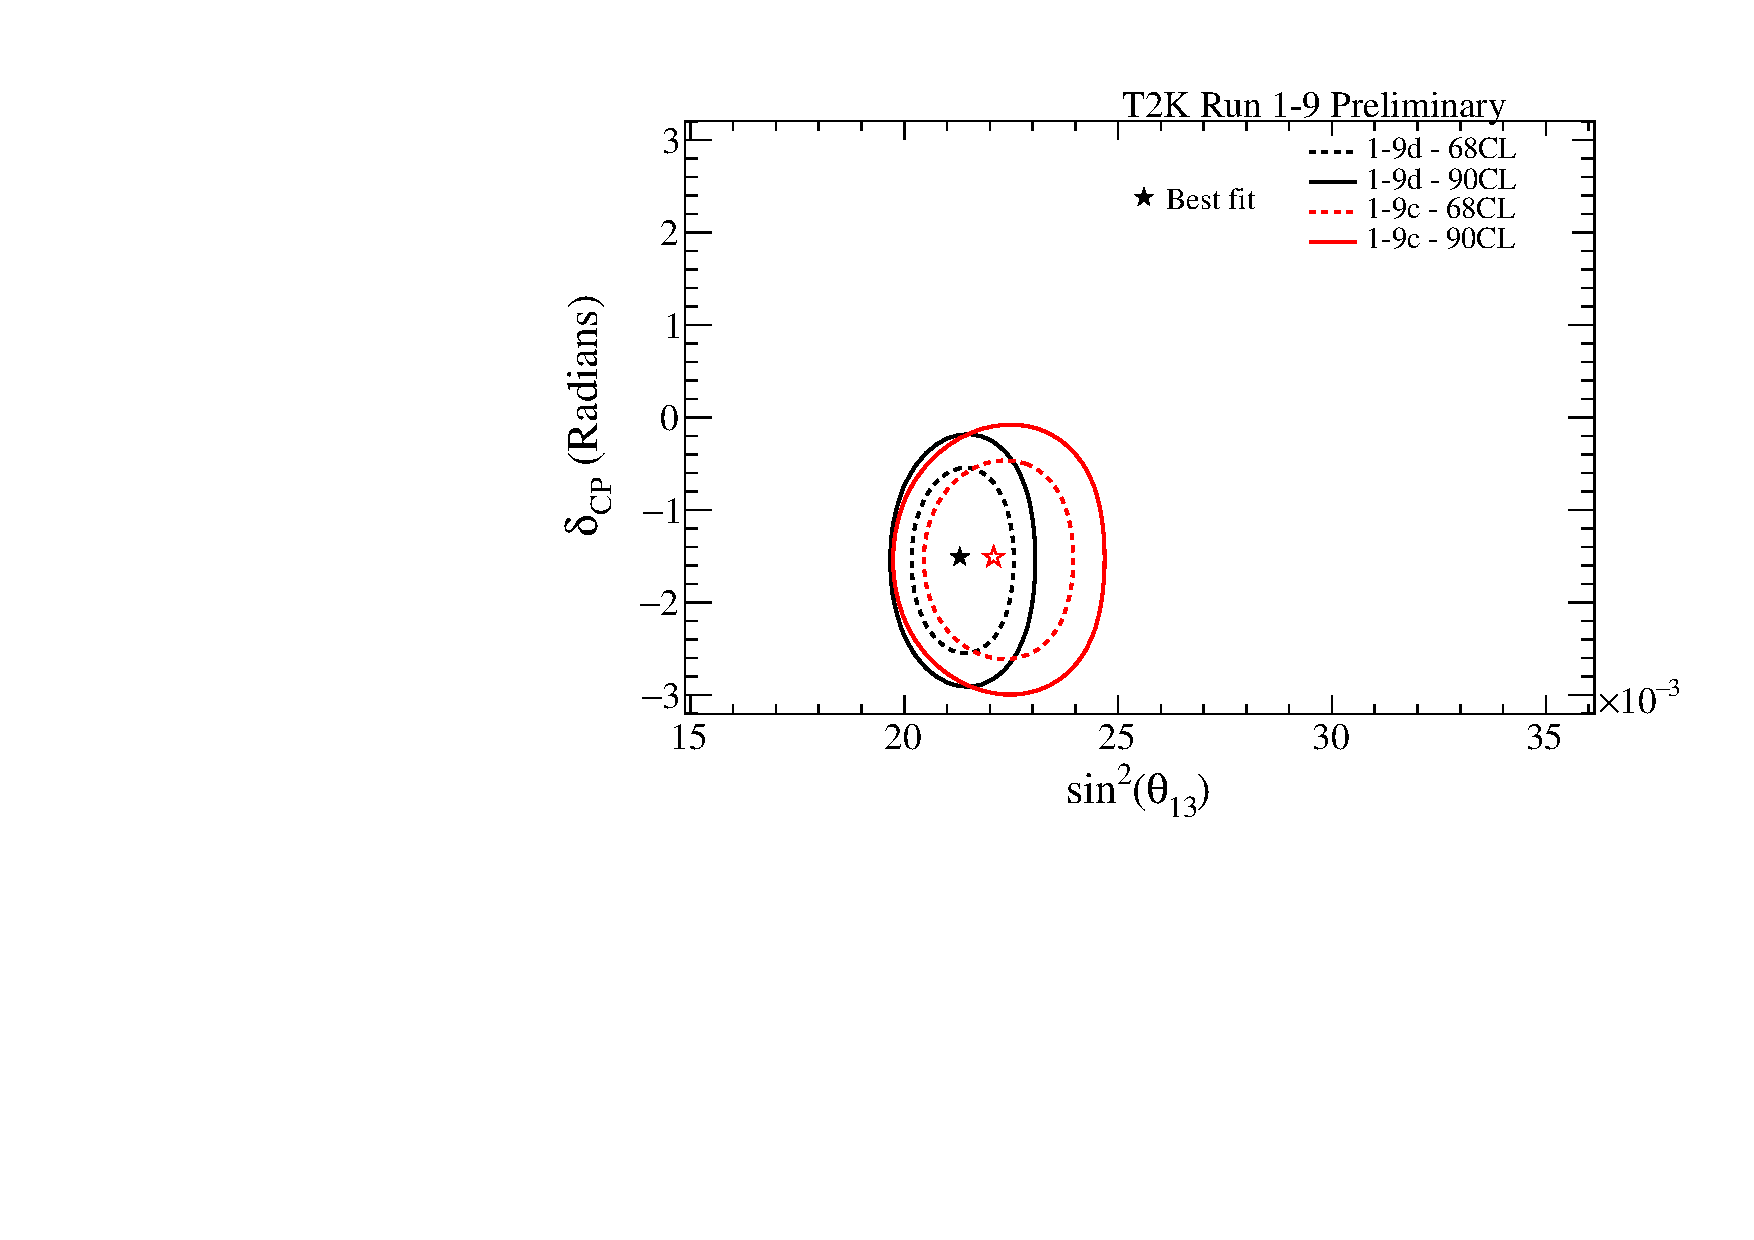
\includegraphics[width=0.9\textwidth]{images/sensitivity/comparison/appearance_wrc_inverted_1-9d_v_1-9c}
		\caption{\appearance IH with reactor constraint}
	\end{subfigure}
	\begin{subfigure}[b]{0.49\textwidth}
		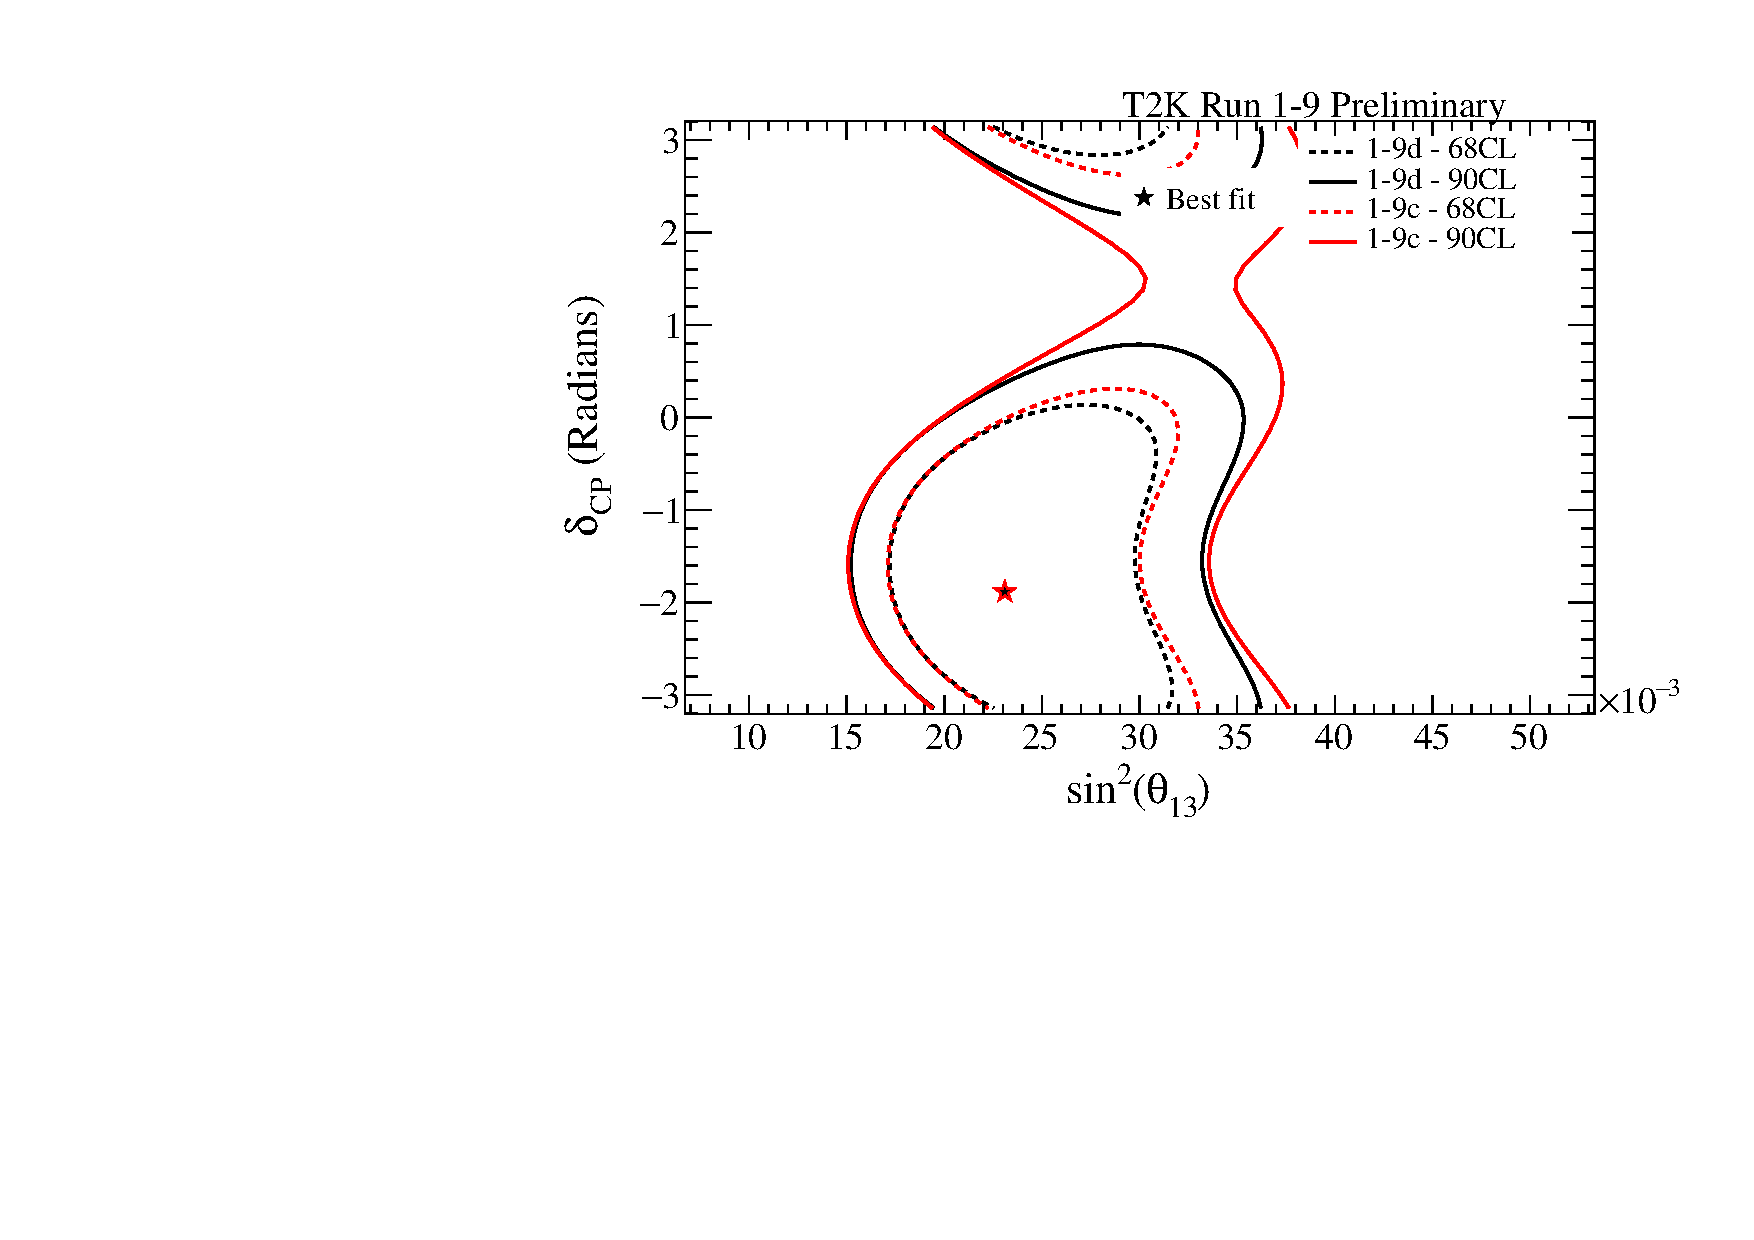
\includegraphics[width=0.9\textwidth]{images/sensitivity/comparison/appearance_worc_normal_1-9d_v_1-9c}
		\caption{\appearance NH without reactor constraint}
	\end{subfigure}
	\begin{subfigure}[b]{0.49\textwidth}
		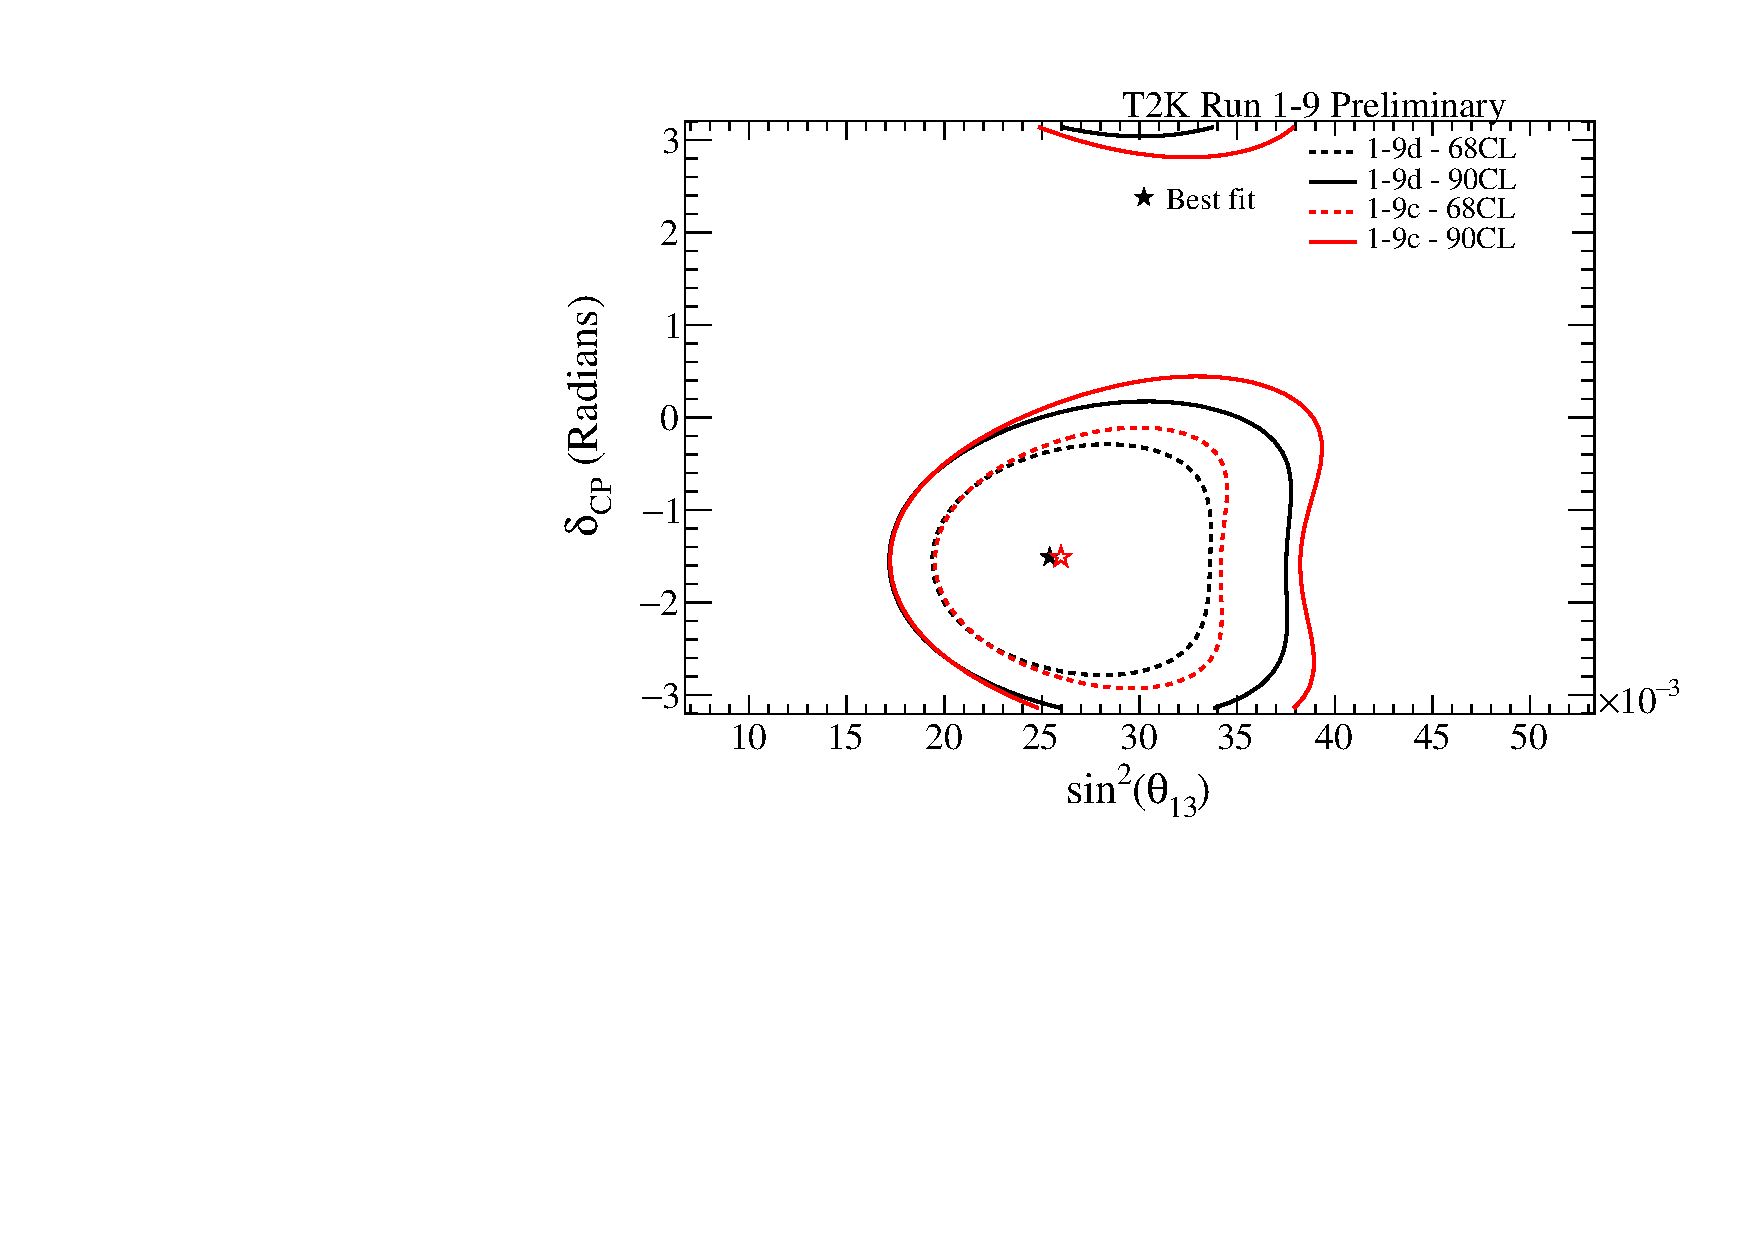
\includegraphics[width=0.9\textwidth]{images/sensitivity/comparison/appearance_worc_inverted_1-9d_v_1-9c}
		\caption{\appearance IH without reactor constraint}
	\end{subfigure}
	\caption {
		Contours at 68\% and 90\% CL for \appearance with and without reactor constraint. Normal and inverted hierarchy contours are independent. All 5 samples were used to produce these fits.
	}
	\label{fig:ssqth13_vs_dcp_asimov_compare}
\end{figure*}
\clearpage

\subsection{Results for \disappearance}

The result for \disappearance with reactor constraint and T2K only is shown in fig.~\ref{fig:ssqth23_vs_dmsq_asimov_compare}.

\begin{figure*}[htb]
	\center
	\begin{subfigure}[b]{0.49\textwidth}
		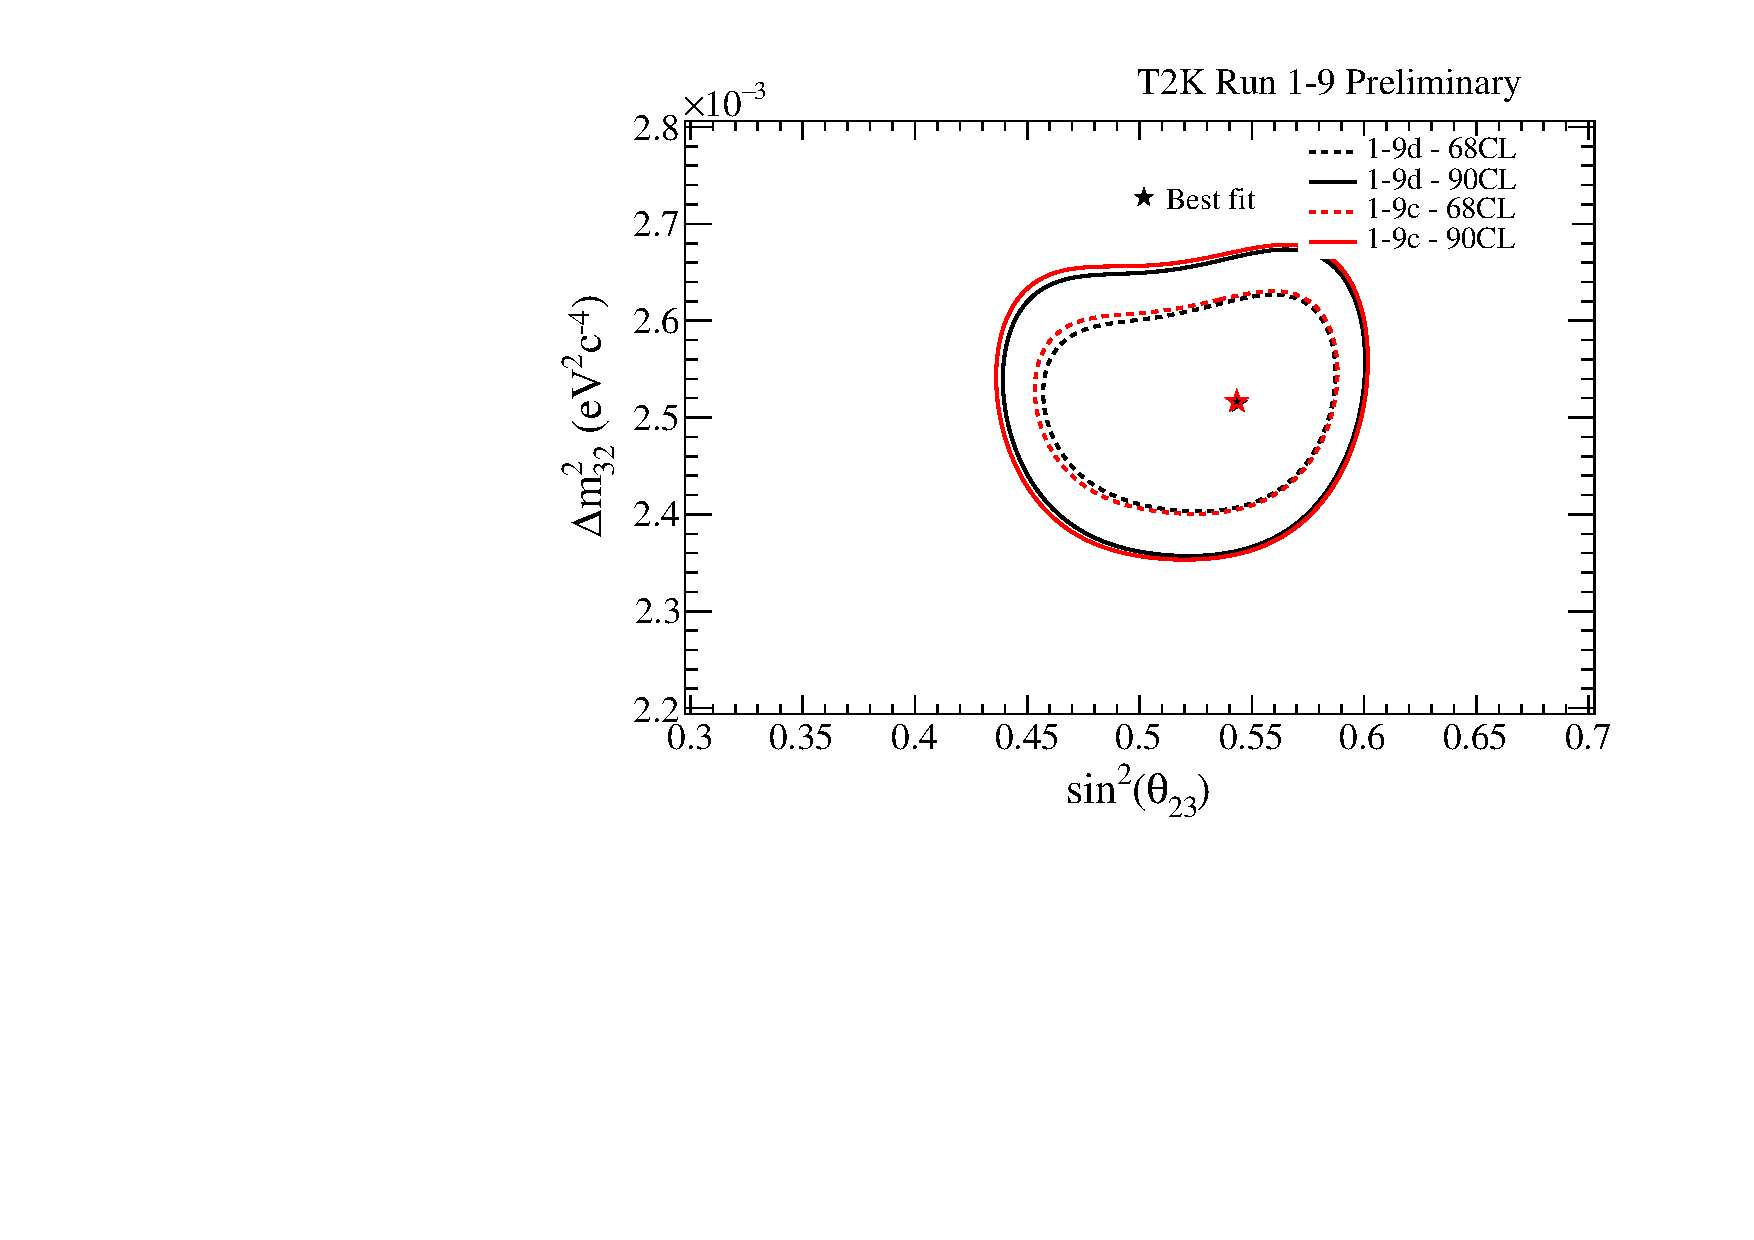
\includegraphics[width=0.9\textwidth]{images/sensitivity/comparison/disappearance_wrc_normal_1-9d_v_1-9c}
		\caption{\disappearance NH with reactor constraint}
	\end{subfigure}
	\begin{subfigure}[b]{0.49\textwidth}
		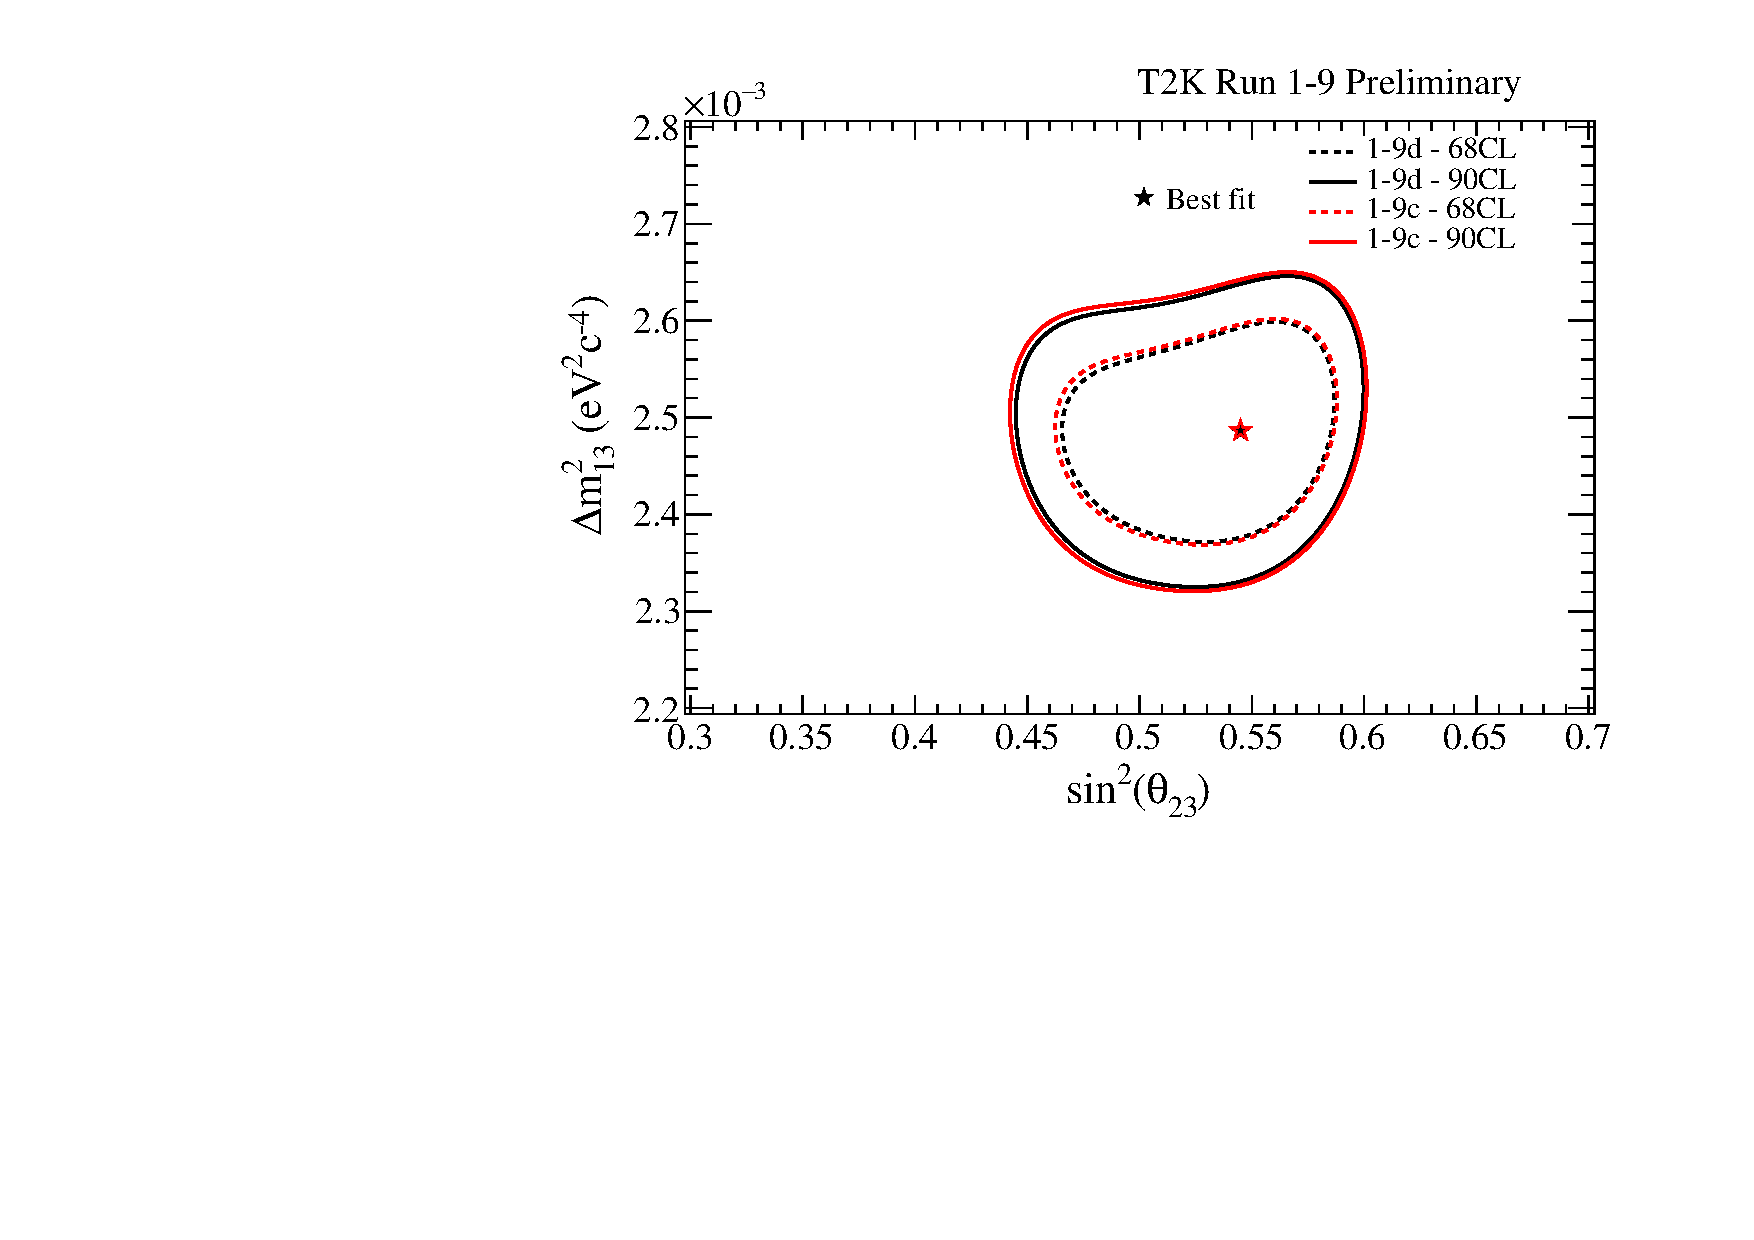
\includegraphics[width=0.9\textwidth]{images/sensitivity/comparison/disappearance_wrc_inverted_1-9d_v_1-9c}
		\caption{\disappearance IH with reactor constraint}
	\end{subfigure}
	\begin{subfigure}[b]{0.49\textwidth}
		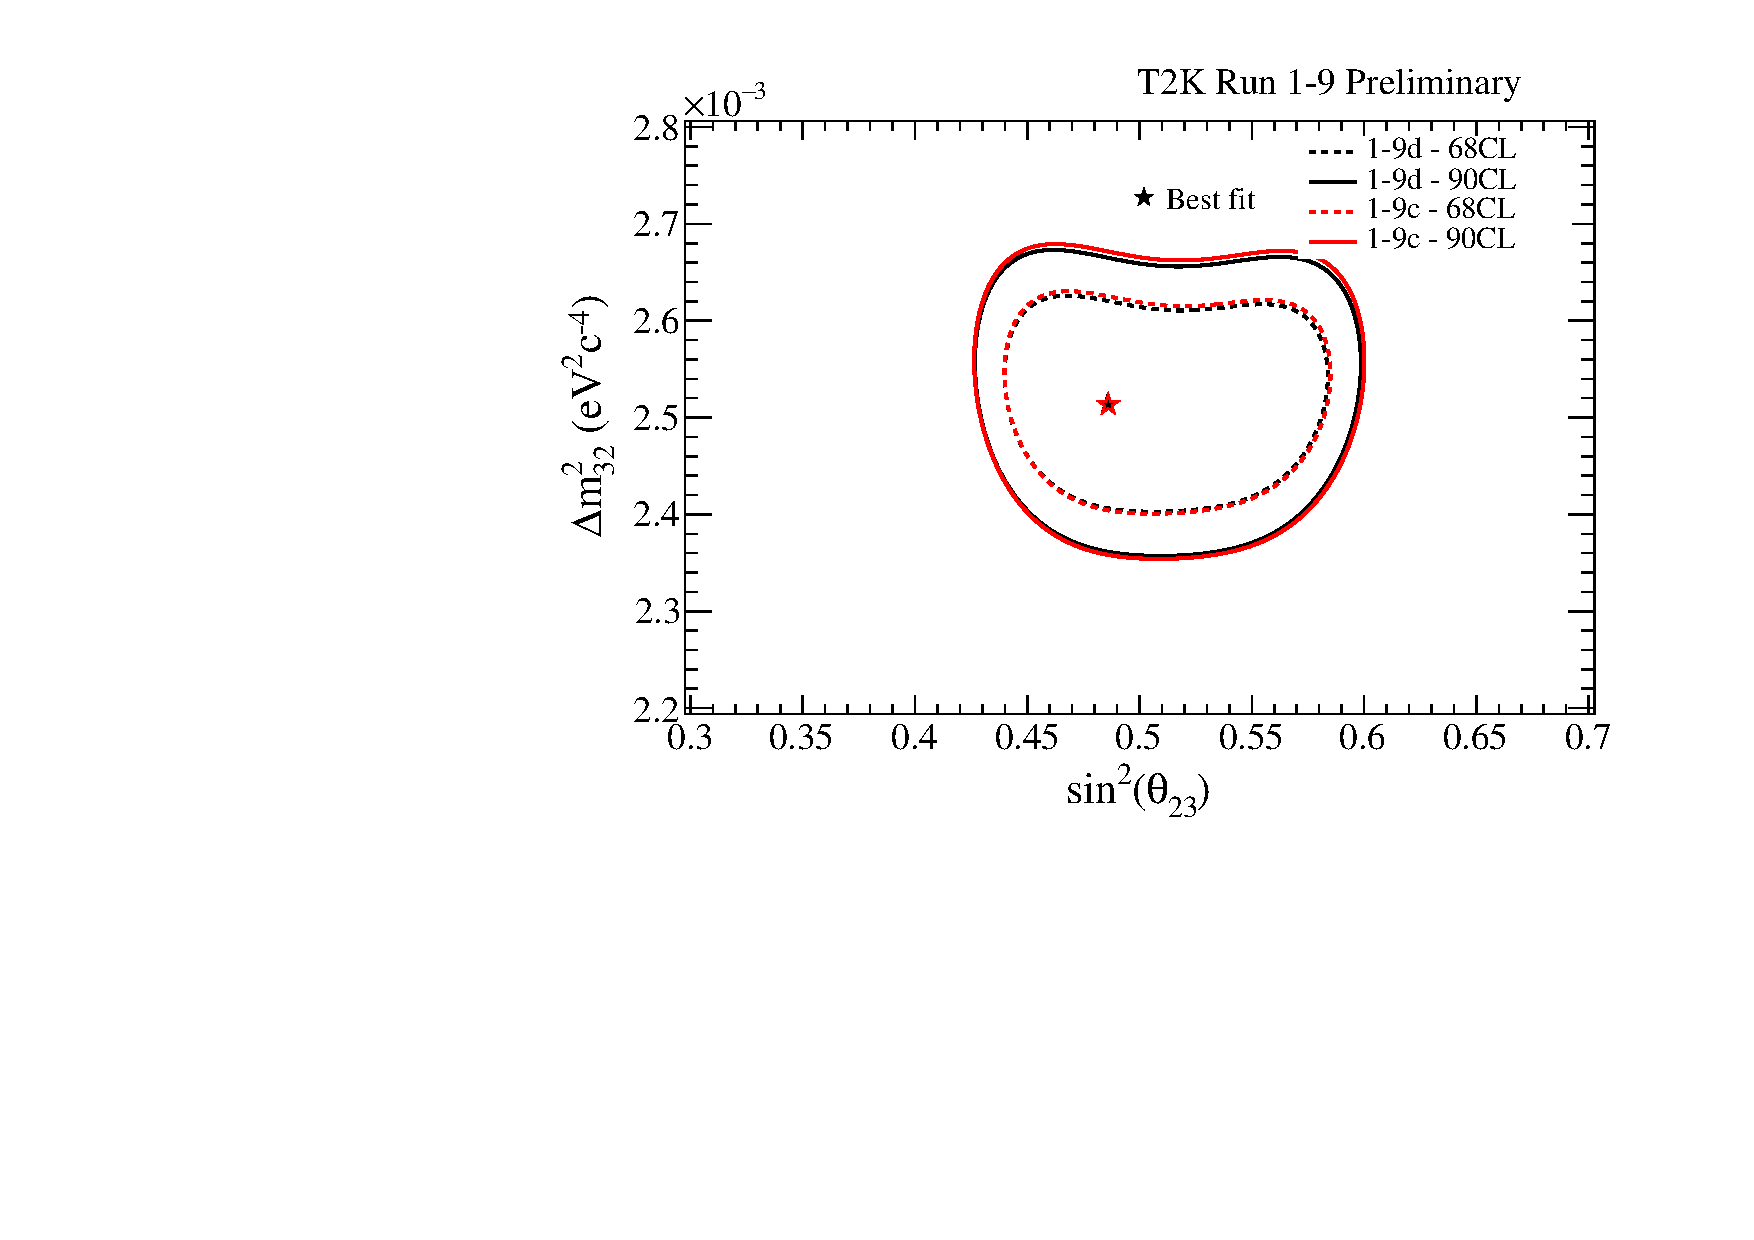
\includegraphics[width=0.9\textwidth]{images/sensitivity/comparison/disappearance_worc_normal_1-9d_v_1-9c}
		\caption{\disappearance NH without reactor constraint}
	\end{subfigure}
	\begin{subfigure}[b]{0.49\textwidth}
		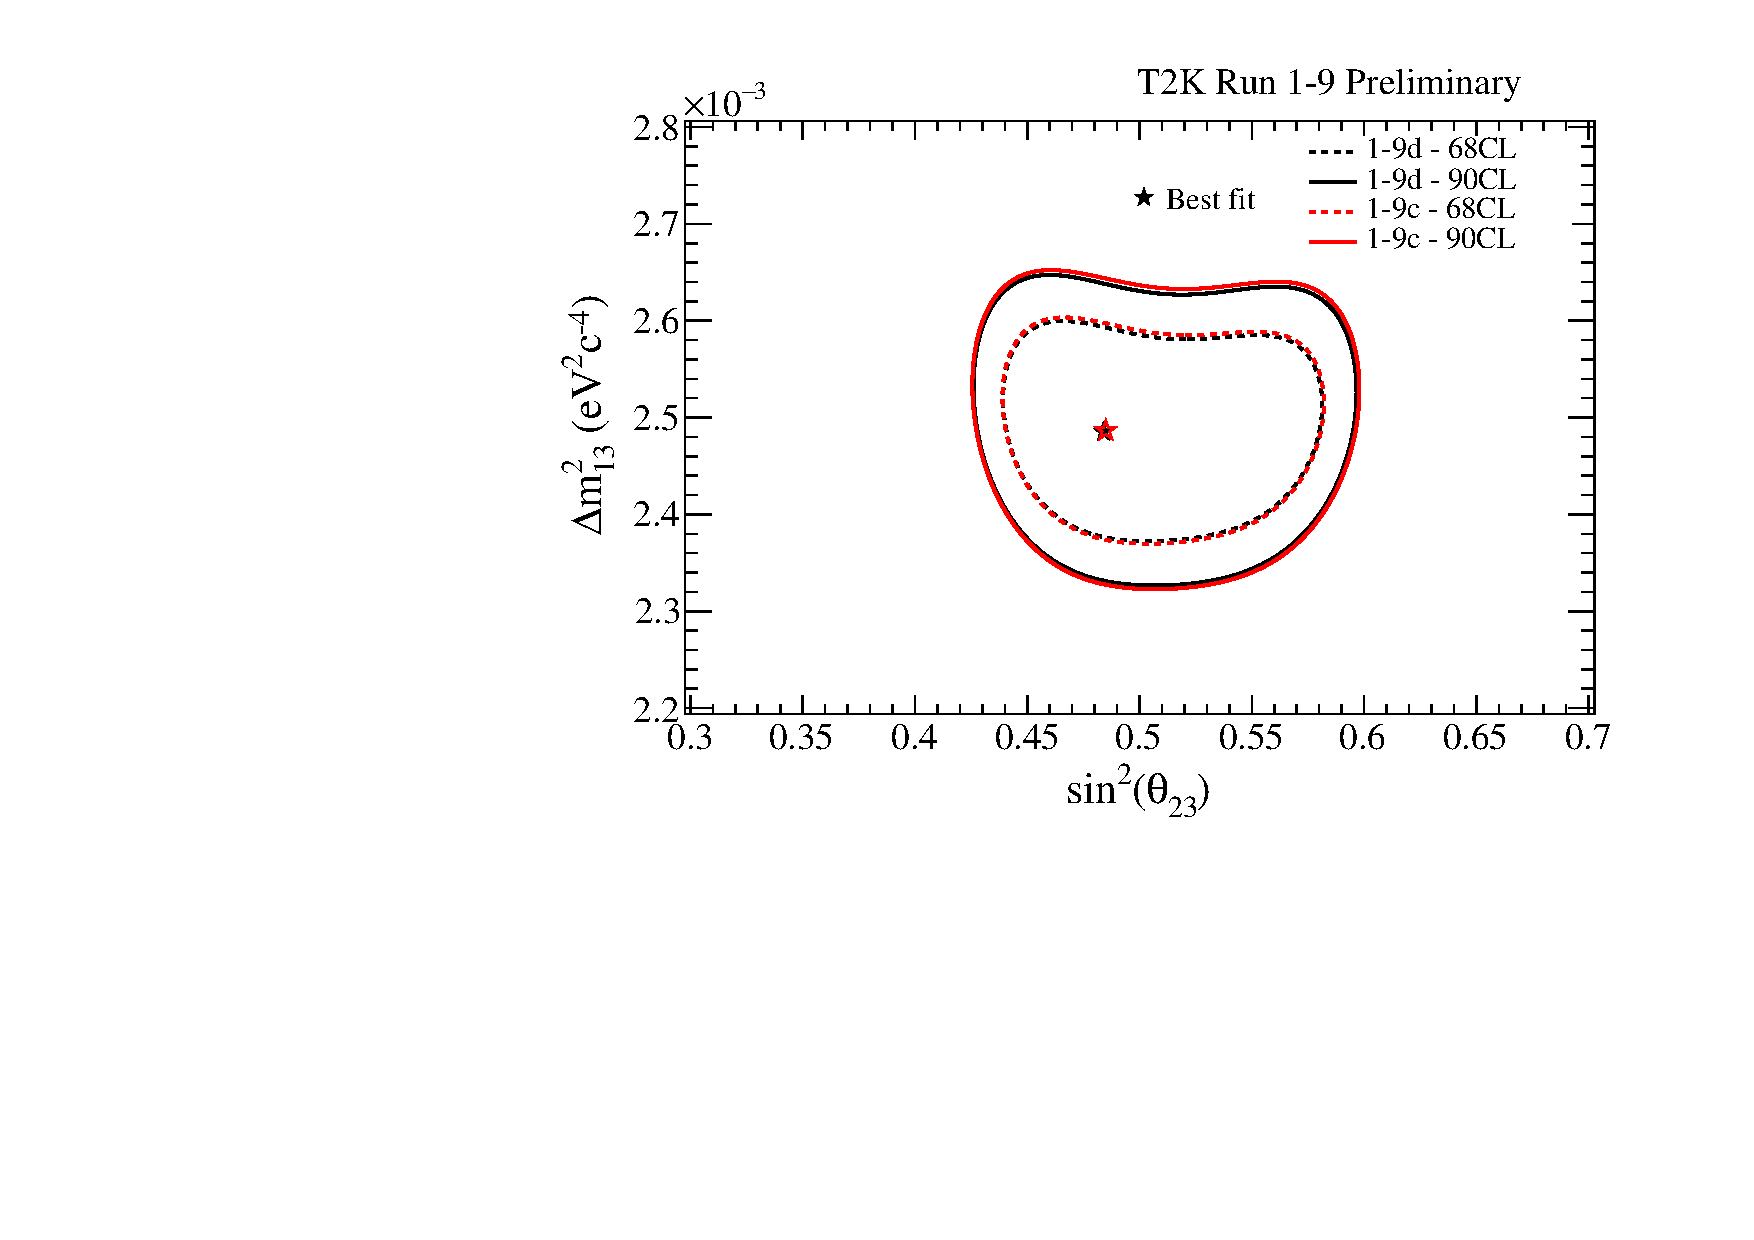
\includegraphics[width=0.9\textwidth]{images/sensitivity/comparison/disappearance_worc_inverted_1-9d_v_1-9c}
		\caption{\disappearance IH without reactor constraint}
	\end{subfigure}
	\caption {
		Contours at 68\% and 90\% CL for \disappearance with and without reactor constraint. Normal and inverted hierarchy contours are independent. All 5 samples were used to produce these fits.
	}
	\label{fig:ssqth23_vs_dmsq_asimov_compare}
\end{figure*}

\clearpage

\subsection{Results for \deltacp}

The result for \deltacp with reactor constraint and T2K only is shown in fig.~\ref{fig:dcp_asimov_compare}.

\begin{figure*}[htb]
	\center
	\begin{subfigure}[b]{0.49\textwidth}
		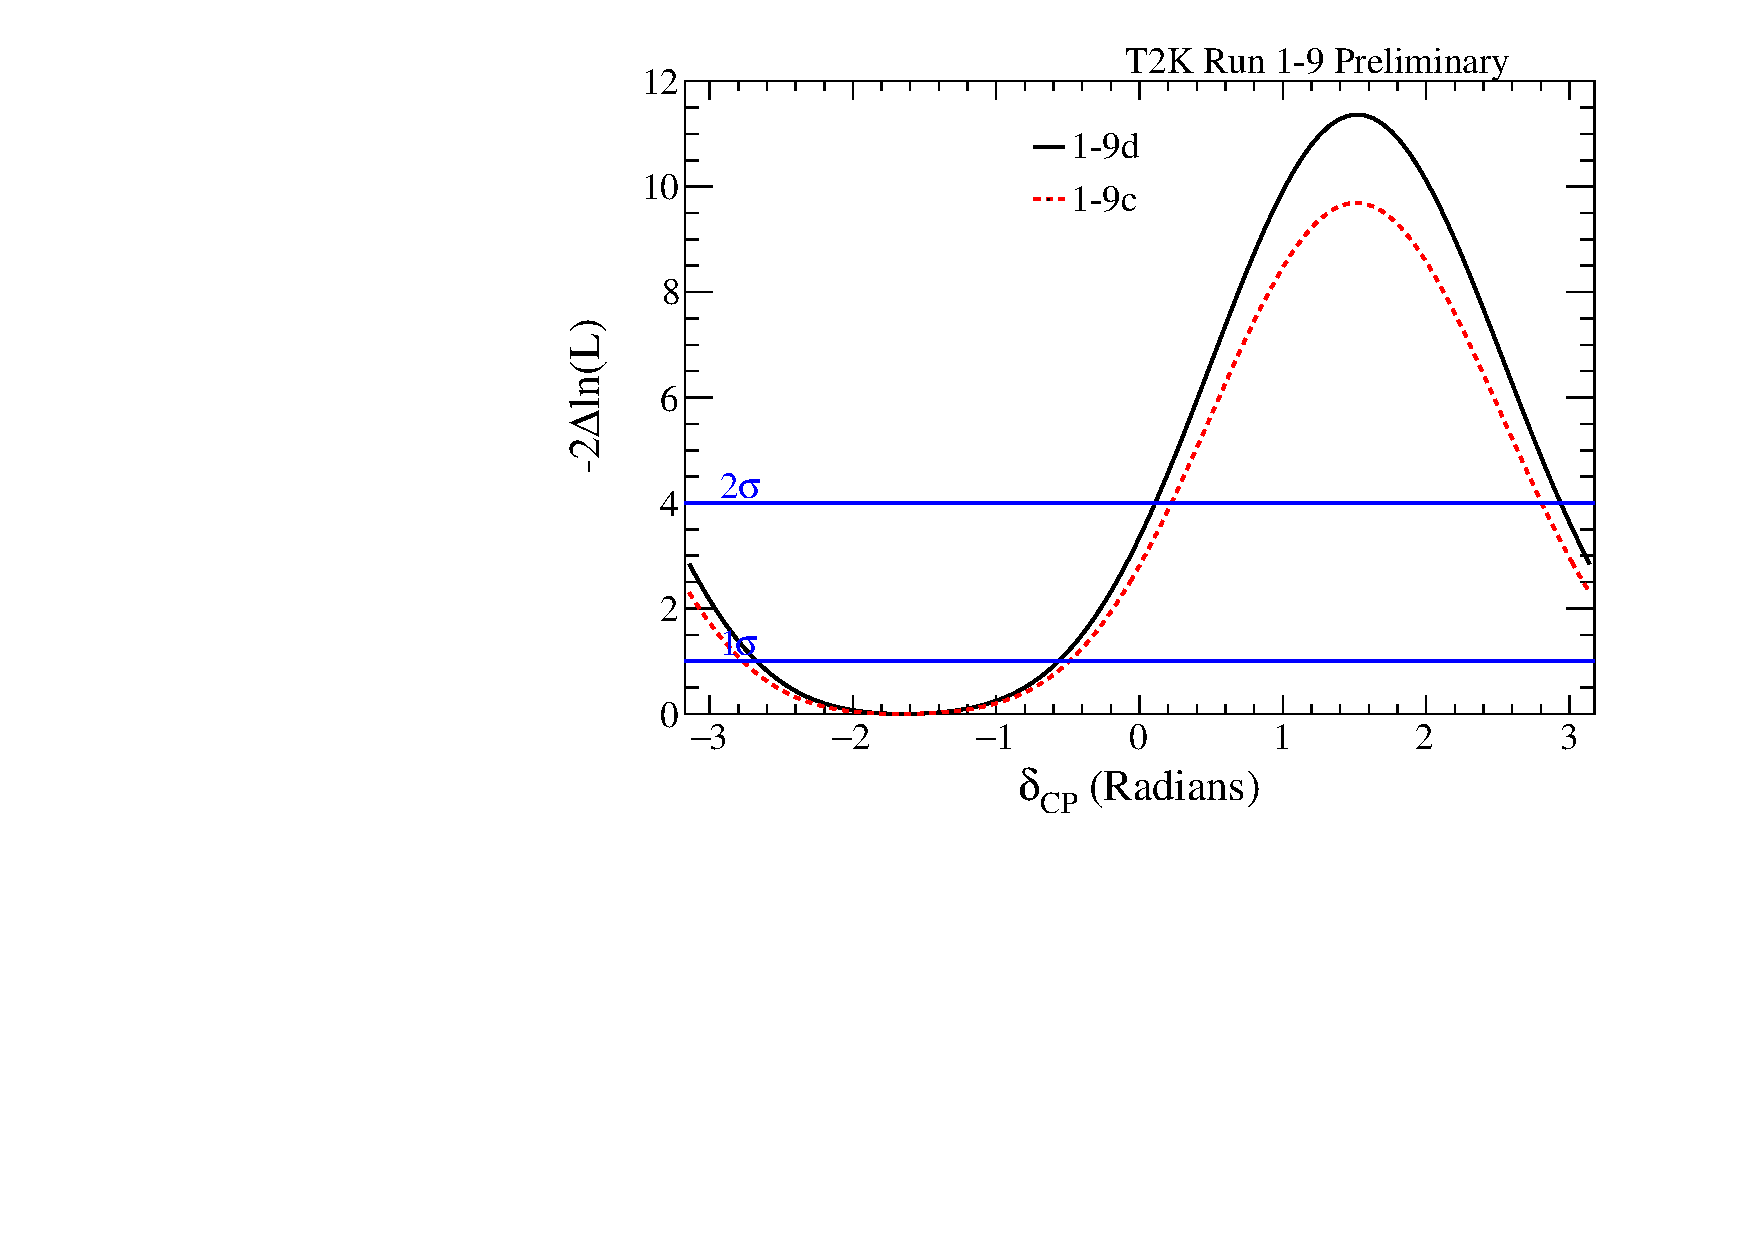
\includegraphics[width=0.9\textwidth]{images/sensitivity/comparison/deltacp_wrc_normal_1-9d_v_1-9c}
		\caption{\deltacp NH with reactor constraint}
	\end{subfigure}
	\begin{subfigure}[b]{0.49\textwidth}
		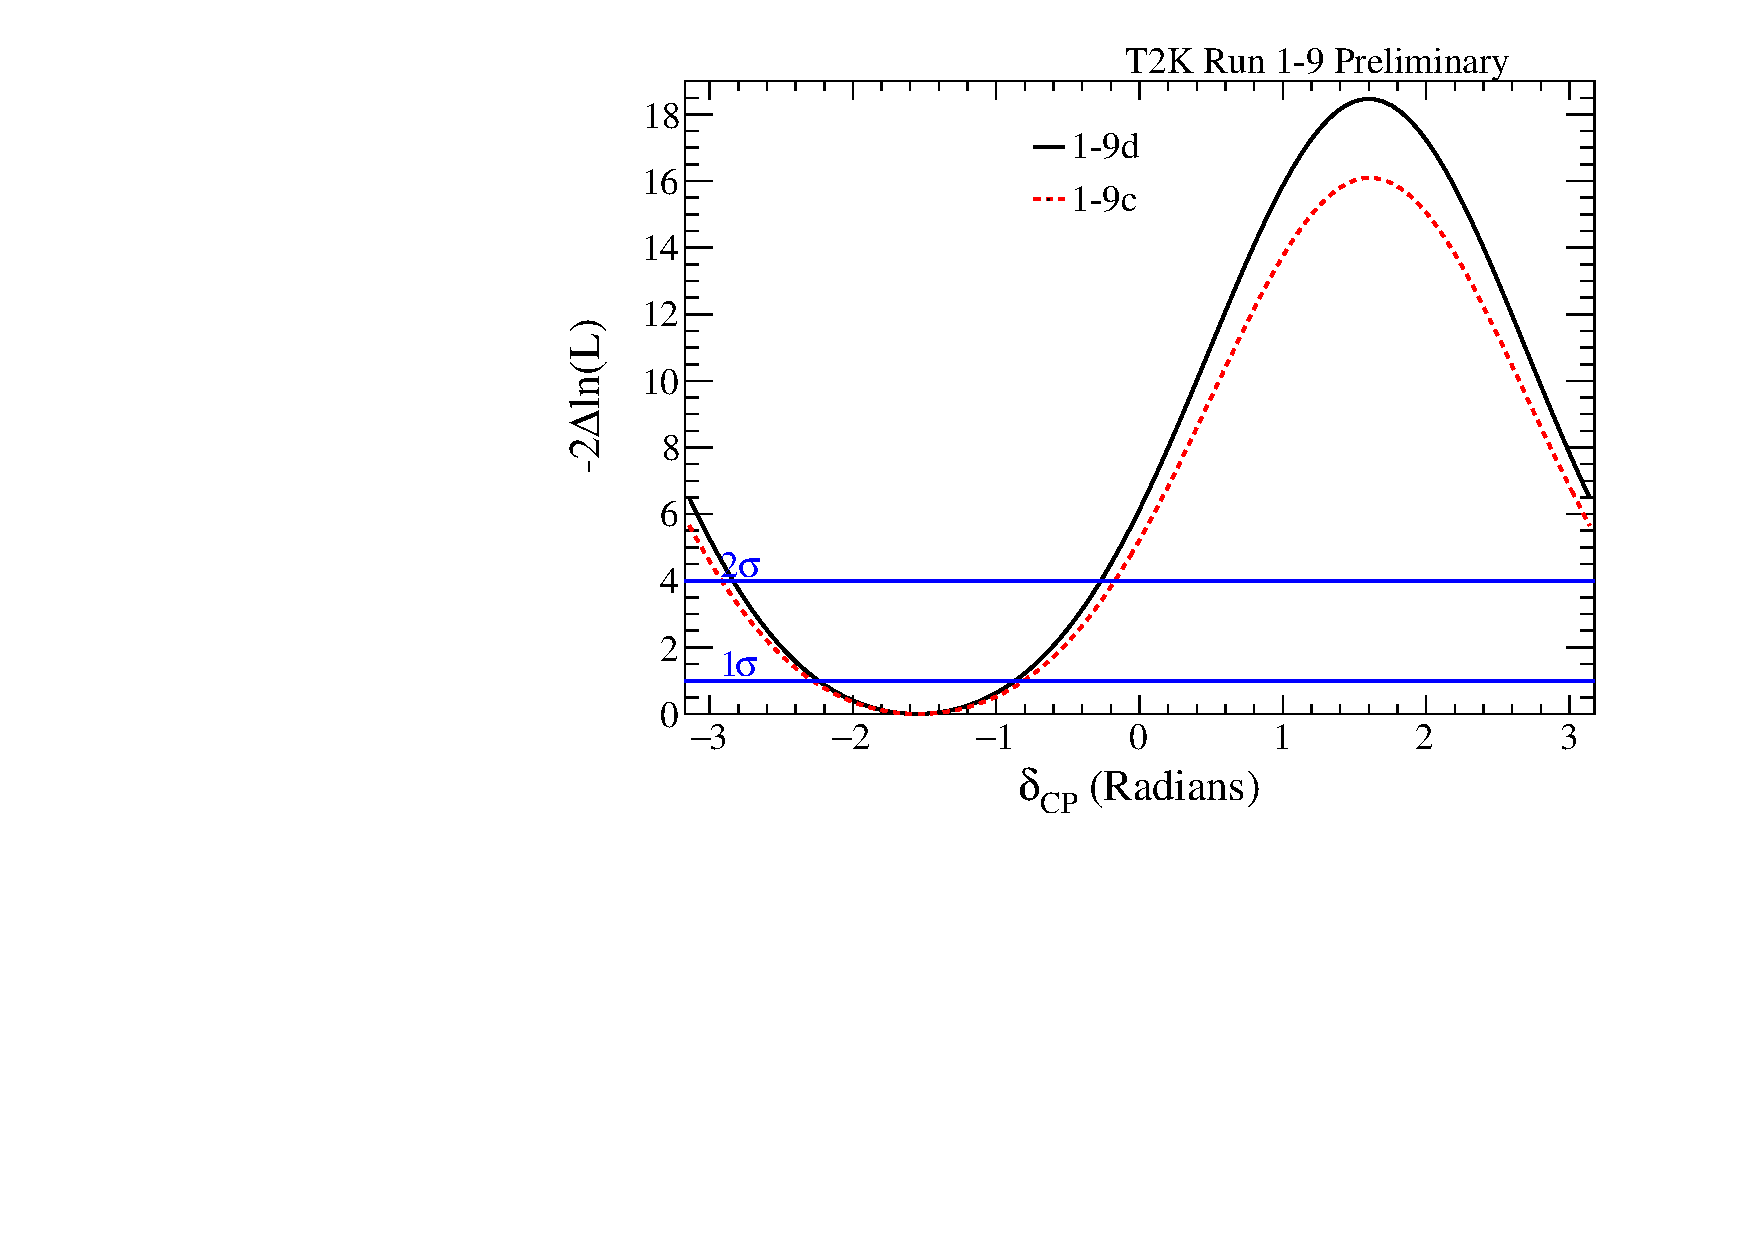
\includegraphics[width=0.9\textwidth]{images/sensitivity/comparison/deltacp_wrc_inverted_1-9d_v_1-9c}
		\caption{\deltacp IH with reactor constraint}
	\end{subfigure}
	\begin{subfigure}[b]{0.49\textwidth}
		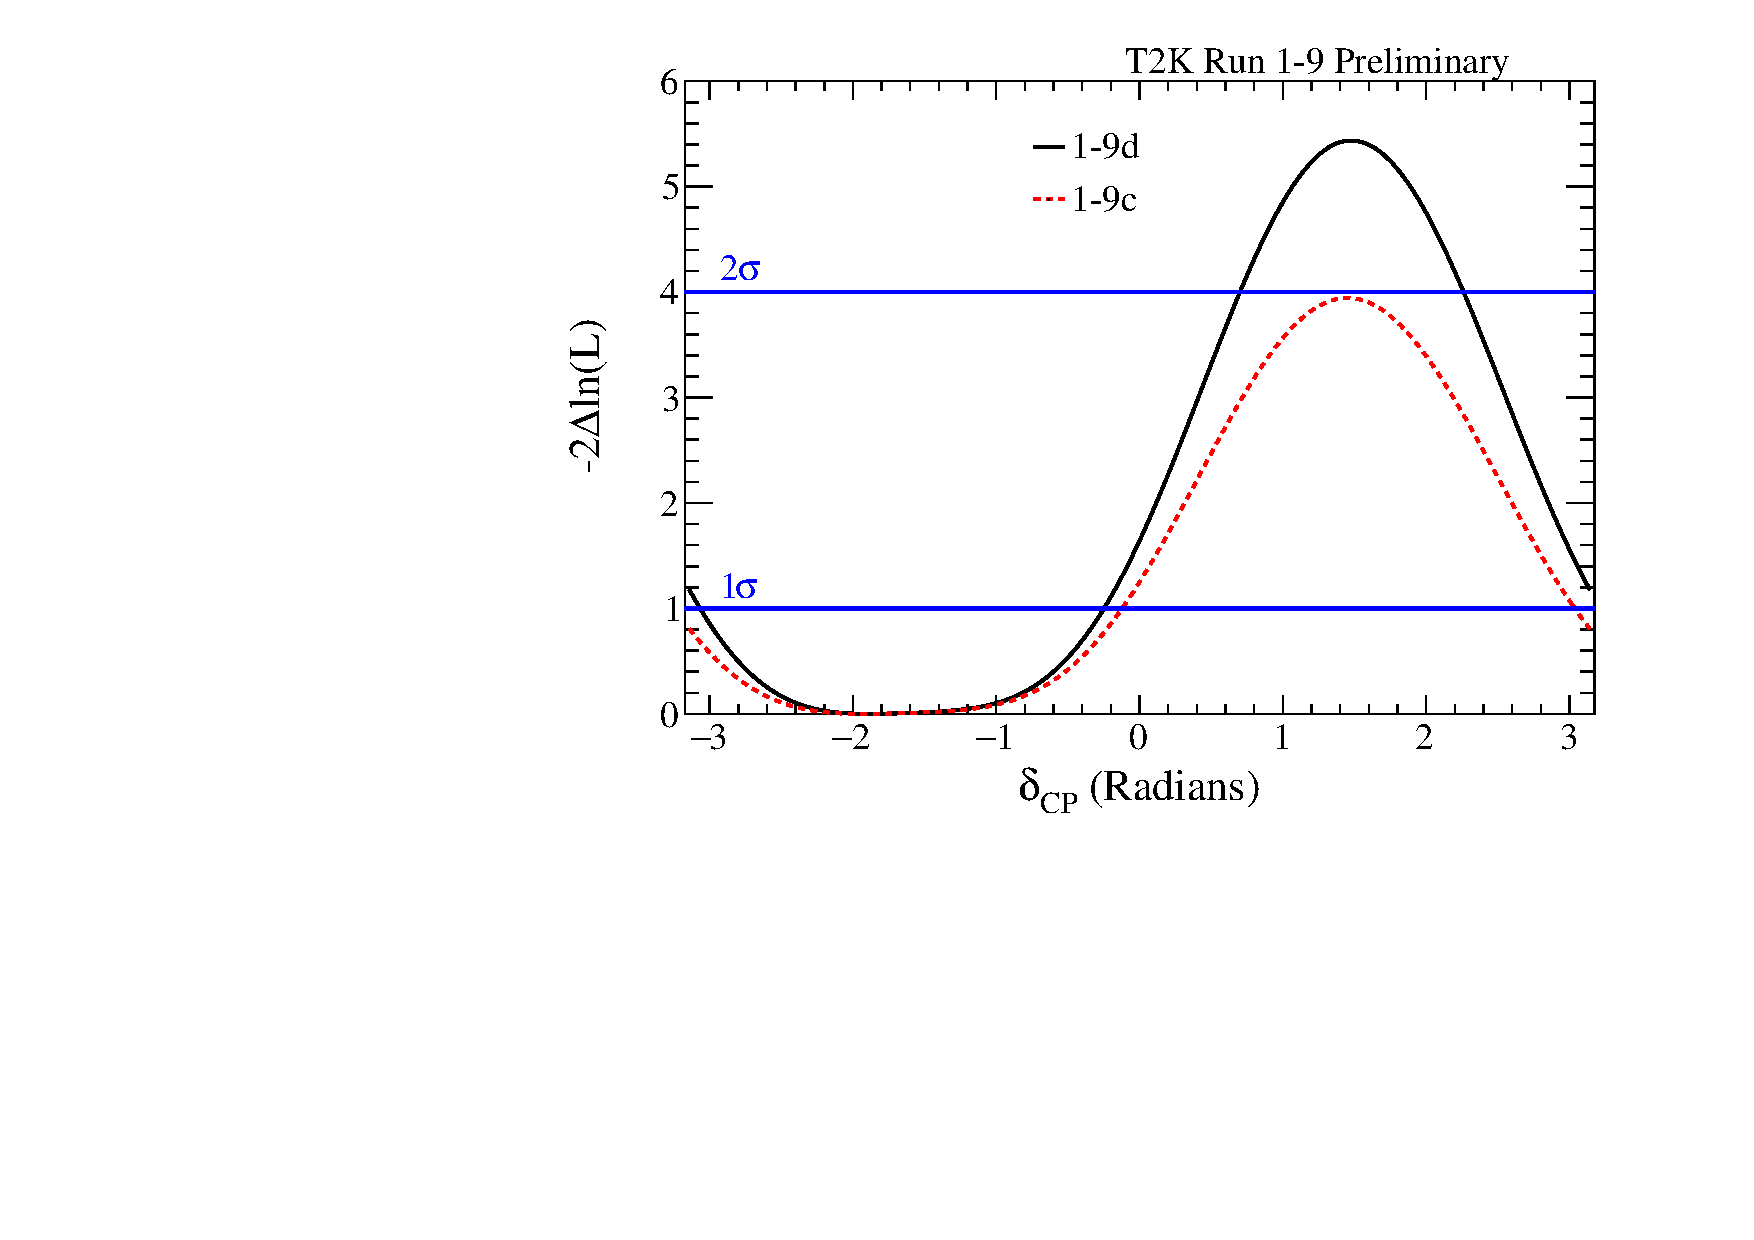
\includegraphics[width=0.9\textwidth]{images/sensitivity/comparison/deltacp_worc_normal_1-9d_v_1-9c}
		\caption{\deltacp NH without reactor constraint}
	\end{subfigure}
	\begin{subfigure}[b]{0.49\textwidth}
		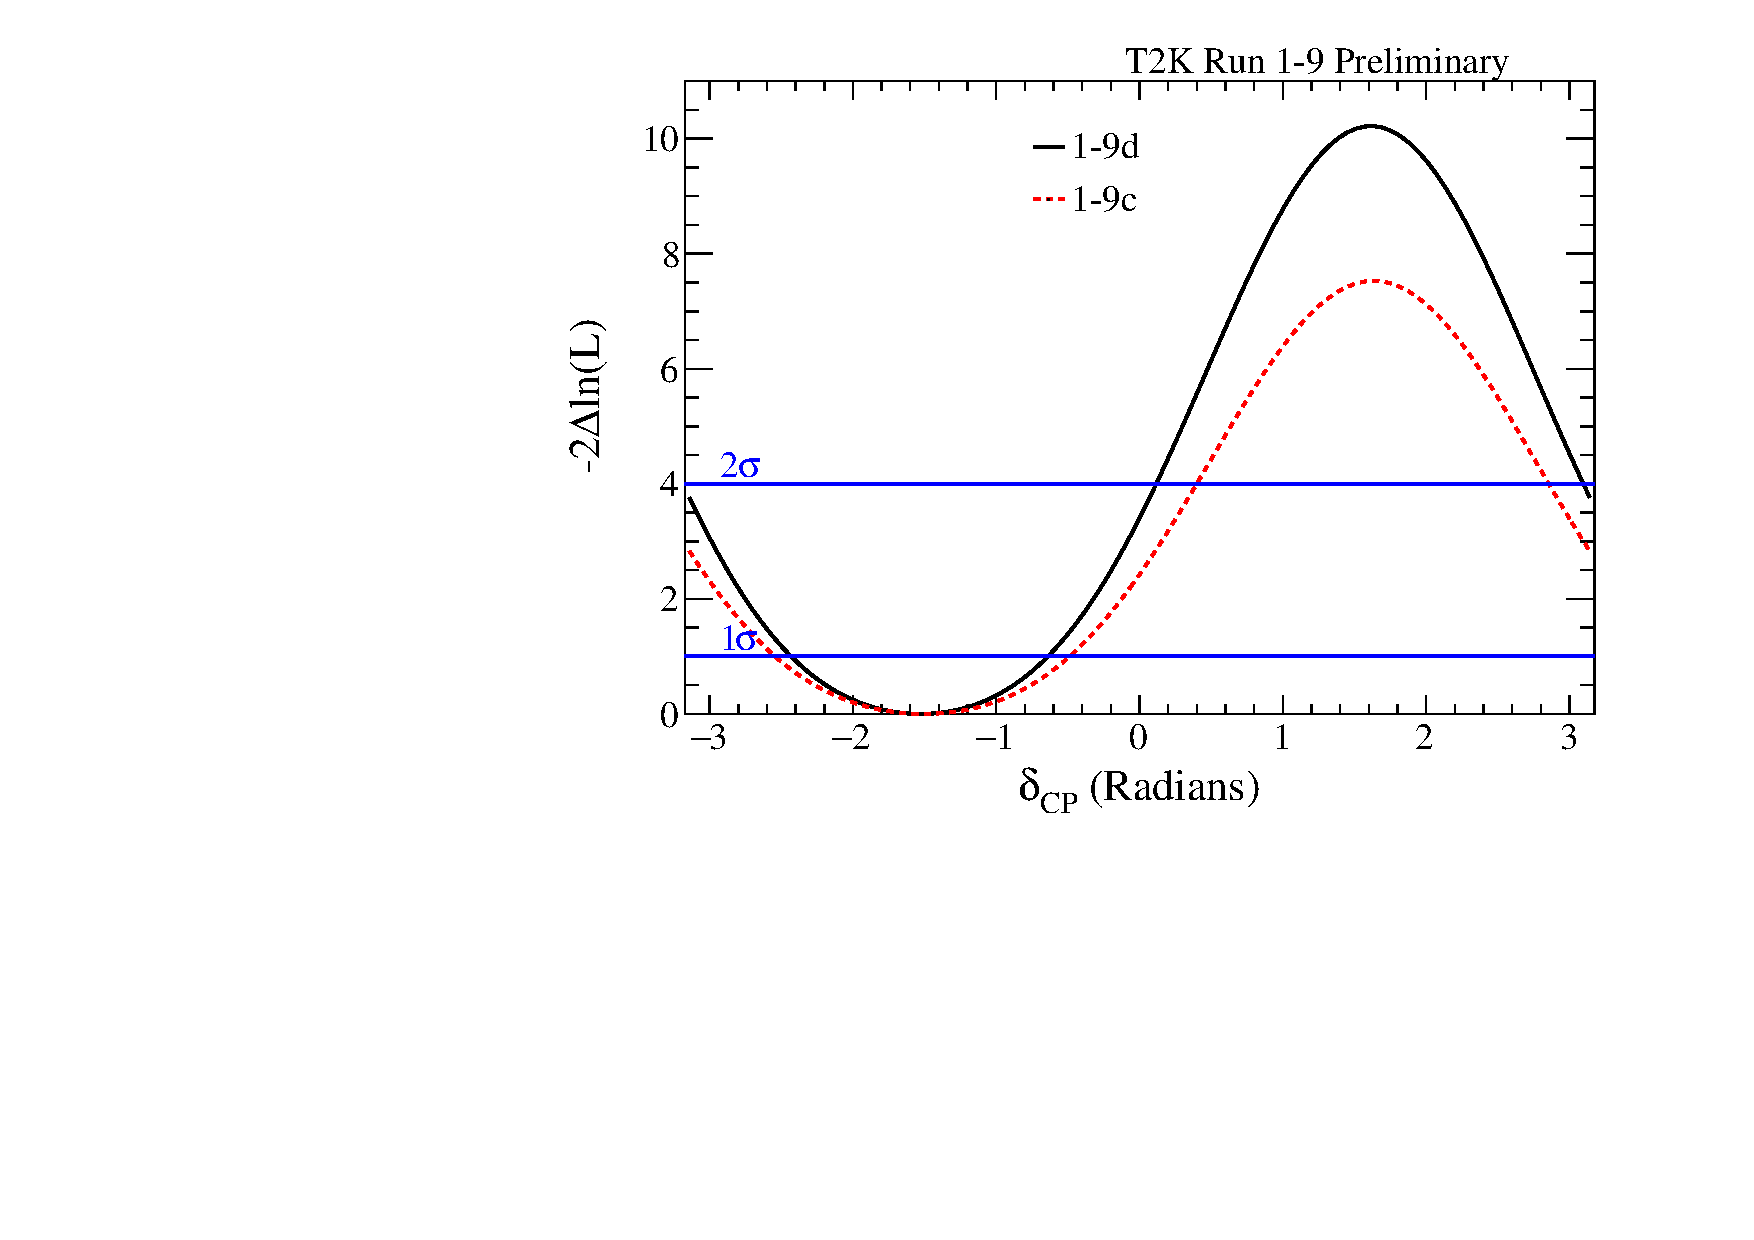
\includegraphics[width=0.9\textwidth]{images/sensitivity/comparison/deltacp_worc_inverted_1-9d_v_1-9c}
		\caption{\deltacp IH without reactor constraint}
	\end{subfigure}
	\caption {
		The expected $\Delta\chi^2$ distribution as a function of \deltacp with and without reactor constraint. Normal and inverted hierarchy contours are independent. All 5 samples were used to produce these fits.
	}
	\label{fig:dcp_asimov_compare}
\end{figure*}
\clearpage

\subsection{Results for \ssqthonethree}

The result for \ssqthonethree (without reactor constraint) is shown in fig.~\ref{fig:th13_asimov_compare}.

\begin{figure*}[htb]
	\center
	\begin{subfigure}[b]{0.49\textwidth}
		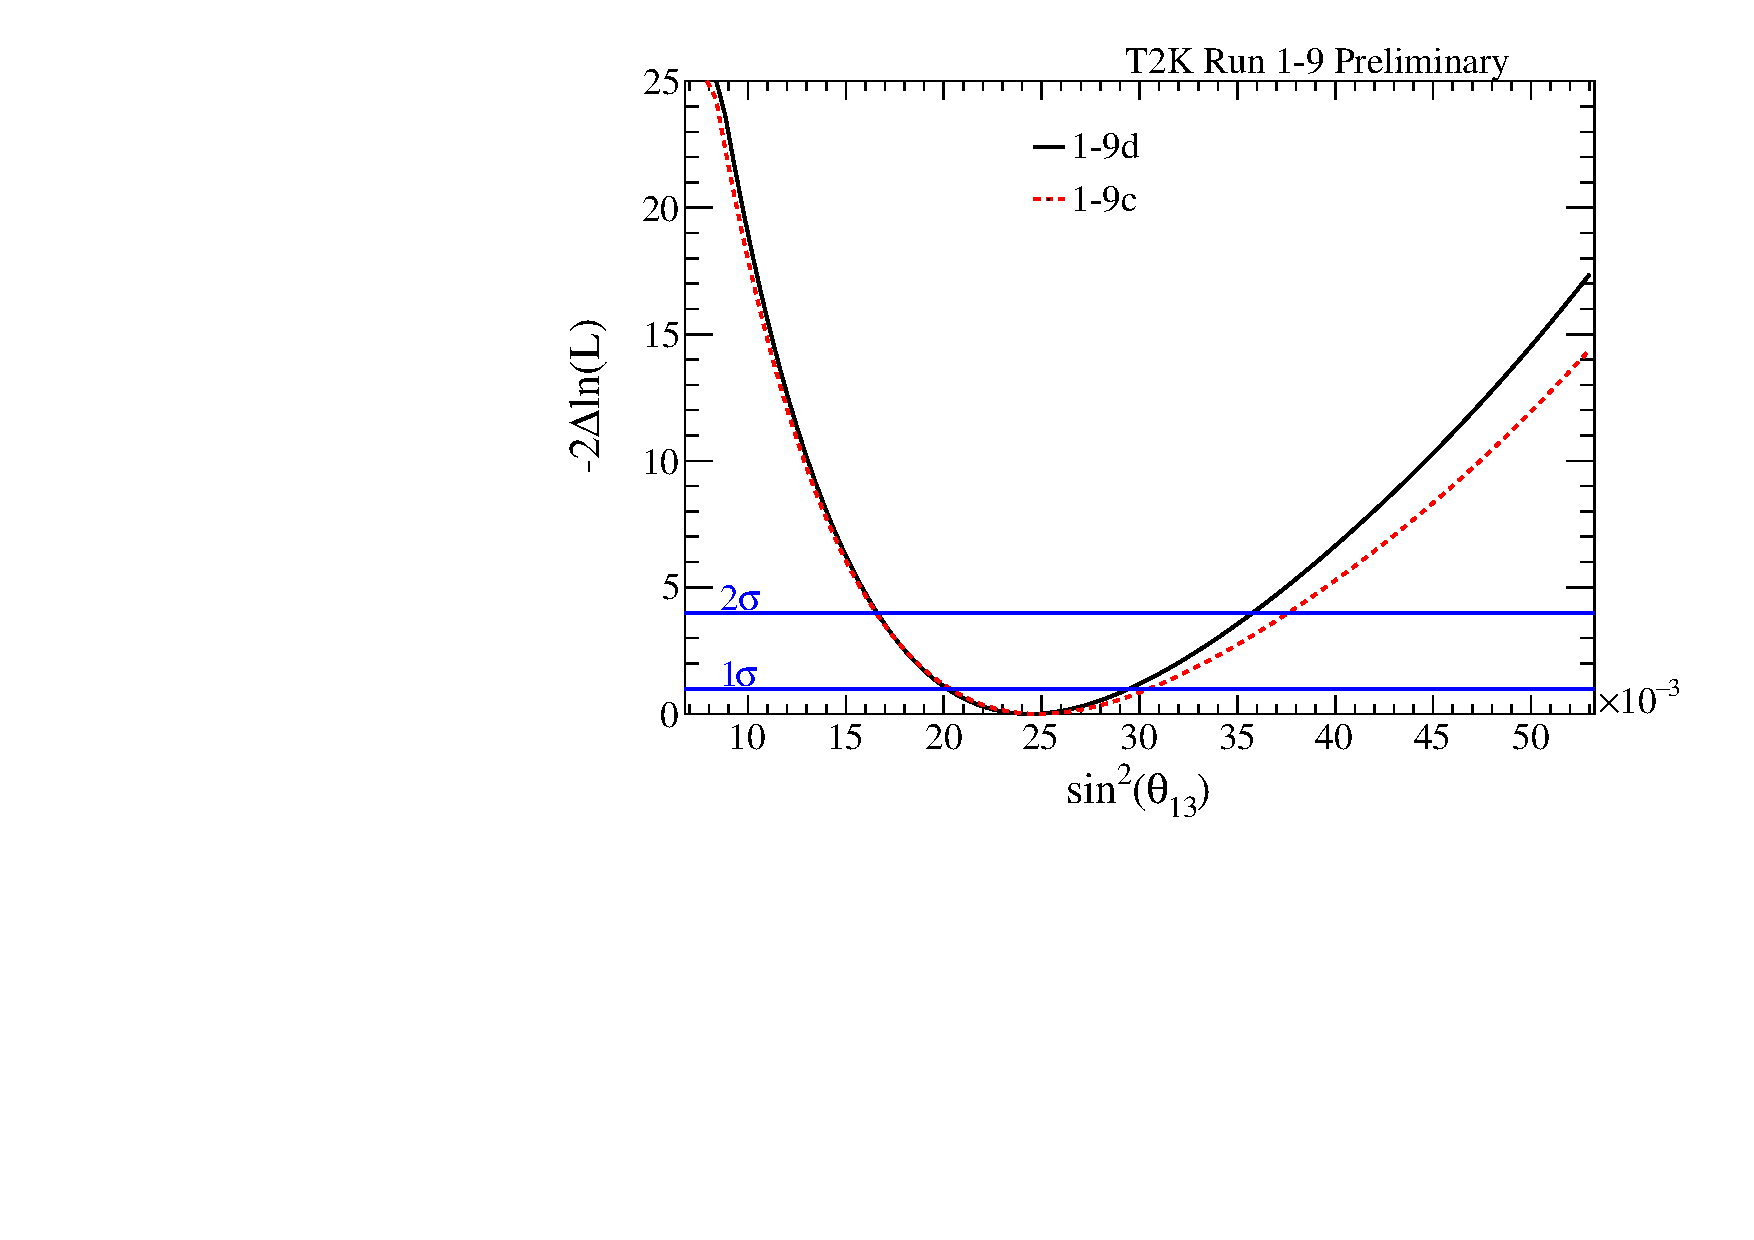
\includegraphics[width=0.9\textwidth]{images/sensitivity/comparison/theta13_worc_normal_1-9d_v_1-9c}
		\caption{\ssqthonethree NH without reactor constraint}
	\end{subfigure}
	\begin{subfigure}[b]{0.49\textwidth}
		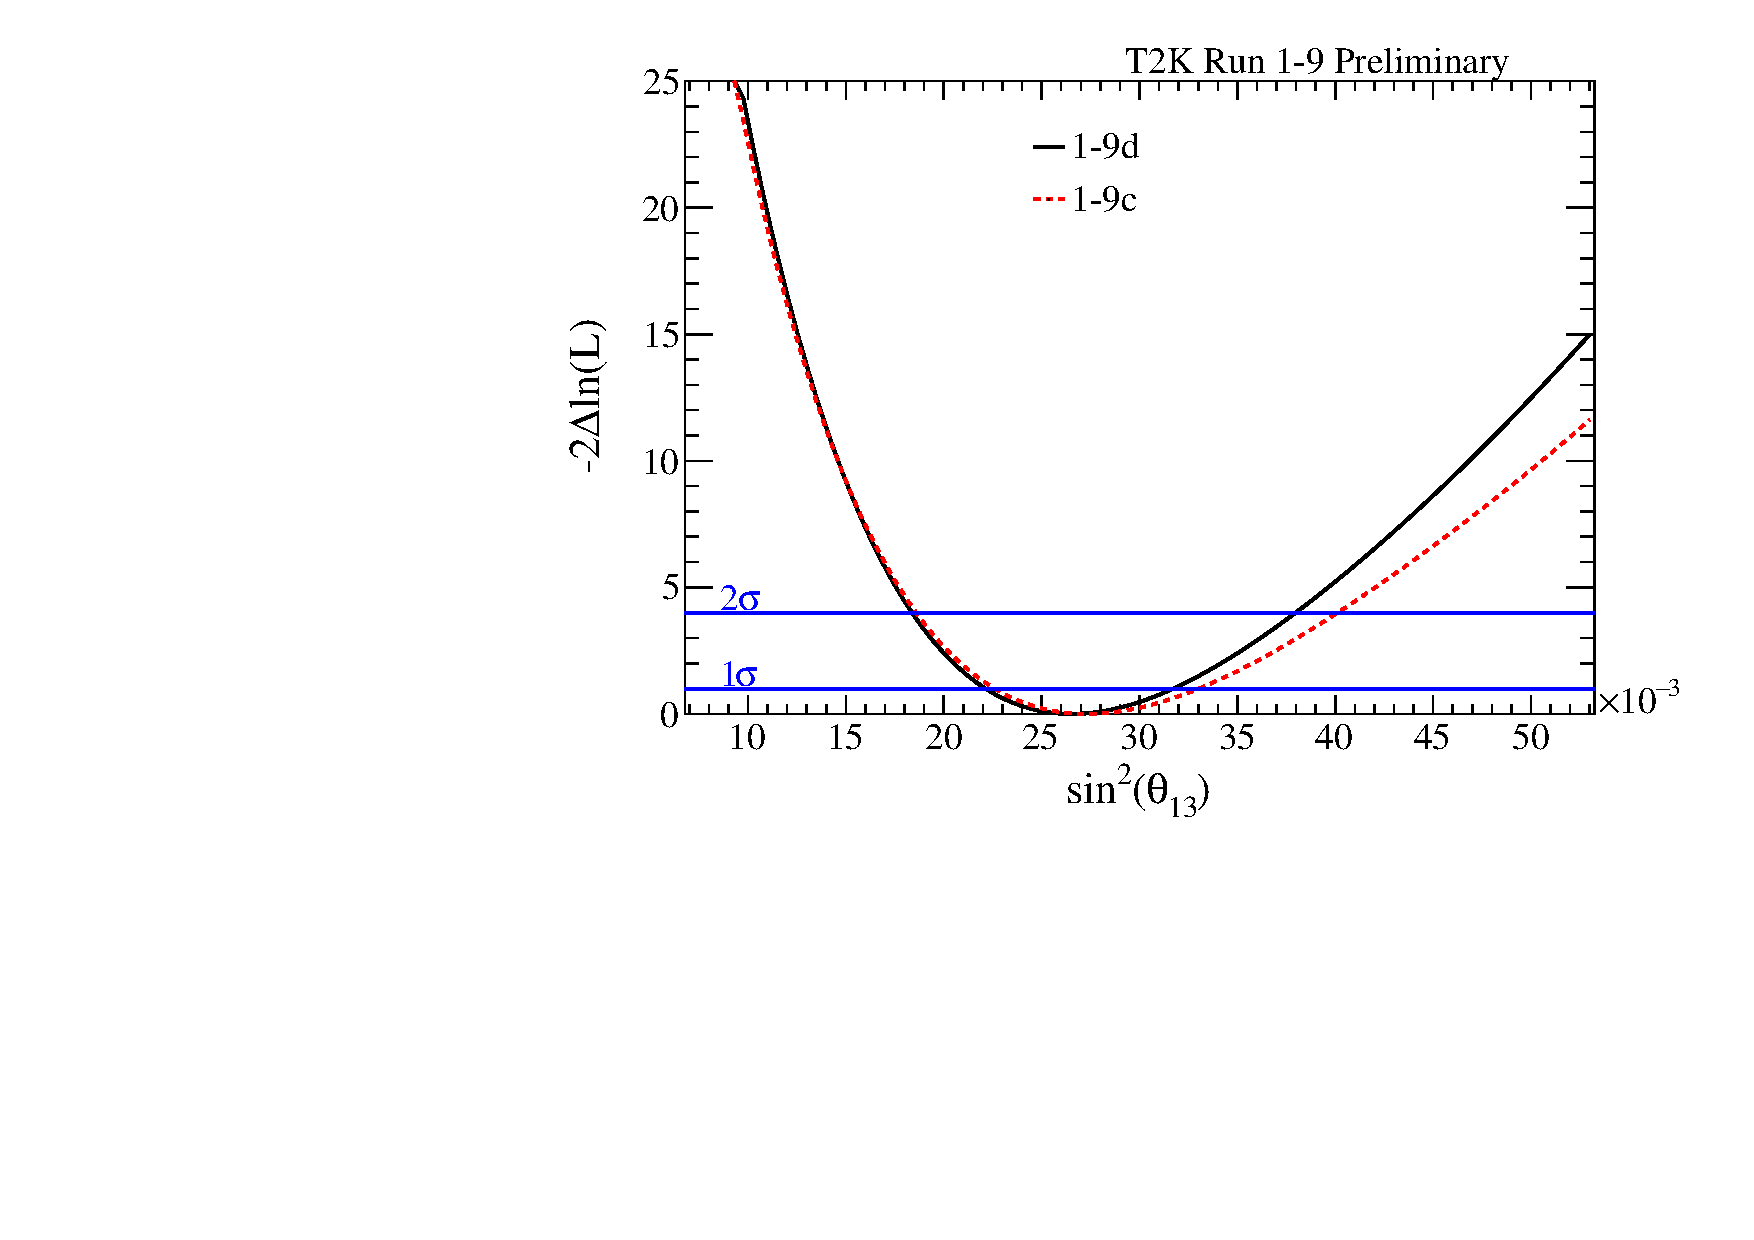
\includegraphics[width=0.9\textwidth]{images/sensitivity/comparison/theta13_worc_inverted_1-9d_v_1-9c}
		\caption{\ssqthonethree IH without reactor constraint}
	\end{subfigure}
	\caption {
		The expected $\Delta\chi^2$ distribution as a function of \ssqthonethree without reactor constraint. Normal and inverted hierarchy contours are independent. All 5 samples were used to produce these fits.
	}
	\label{fig:th13_asimov_compare}
\end{figure*}

\clearpage

\subsection{Results for \ssqthtwothree}

The result for \ssqthtwothree with reactor constraint and T2K only is shown in fig.~\ref{fig:th23_asimov_compare}.

\begin{figure*}[htb]
	\center
	\begin{subfigure}[b]{0.49\textwidth}
		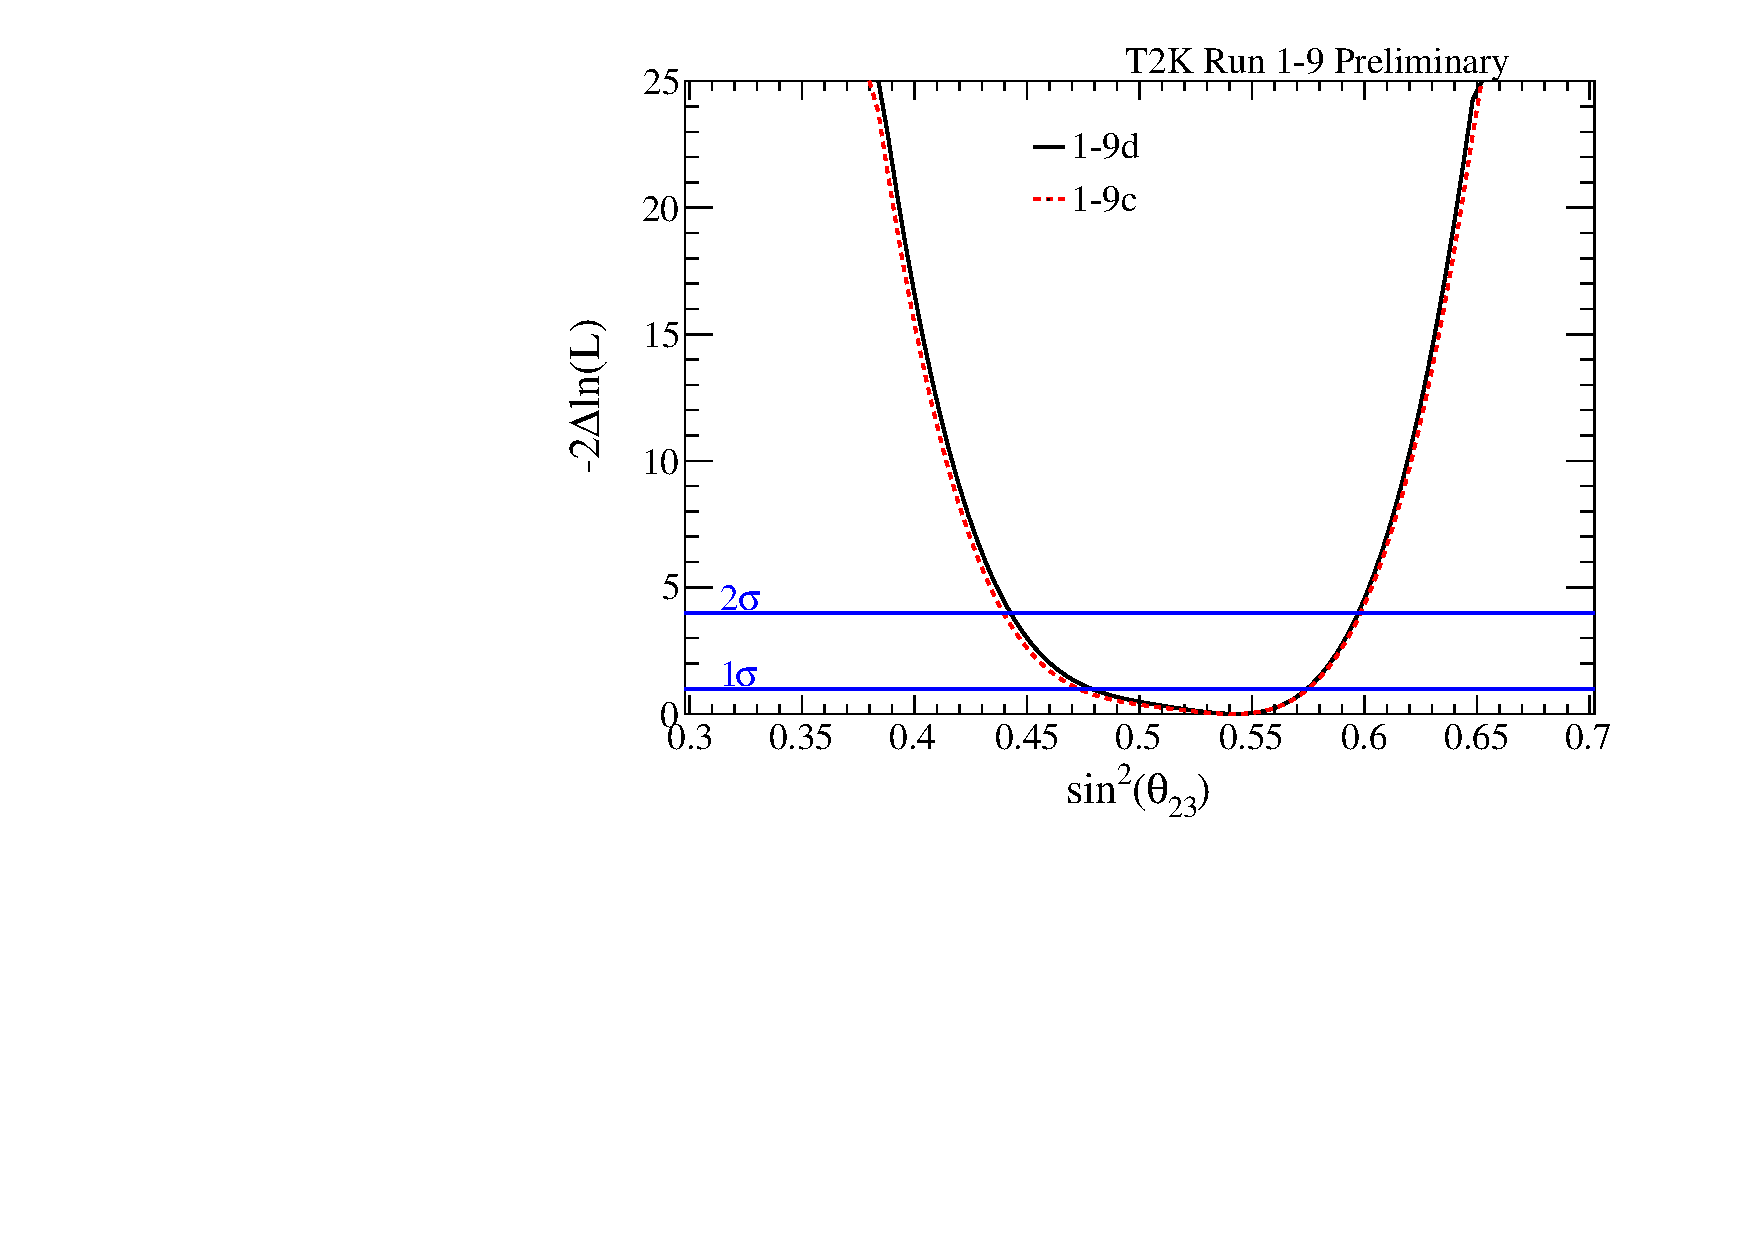
\includegraphics[width=0.9\textwidth]{images/sensitivity/comparison/theta23_wrc_normal_1-9d_v_1-9c}
		\caption{\ssqthtwothree NH with reactor constraint}
	\end{subfigure}
	\begin{subfigure}[b]{0.49\textwidth}
		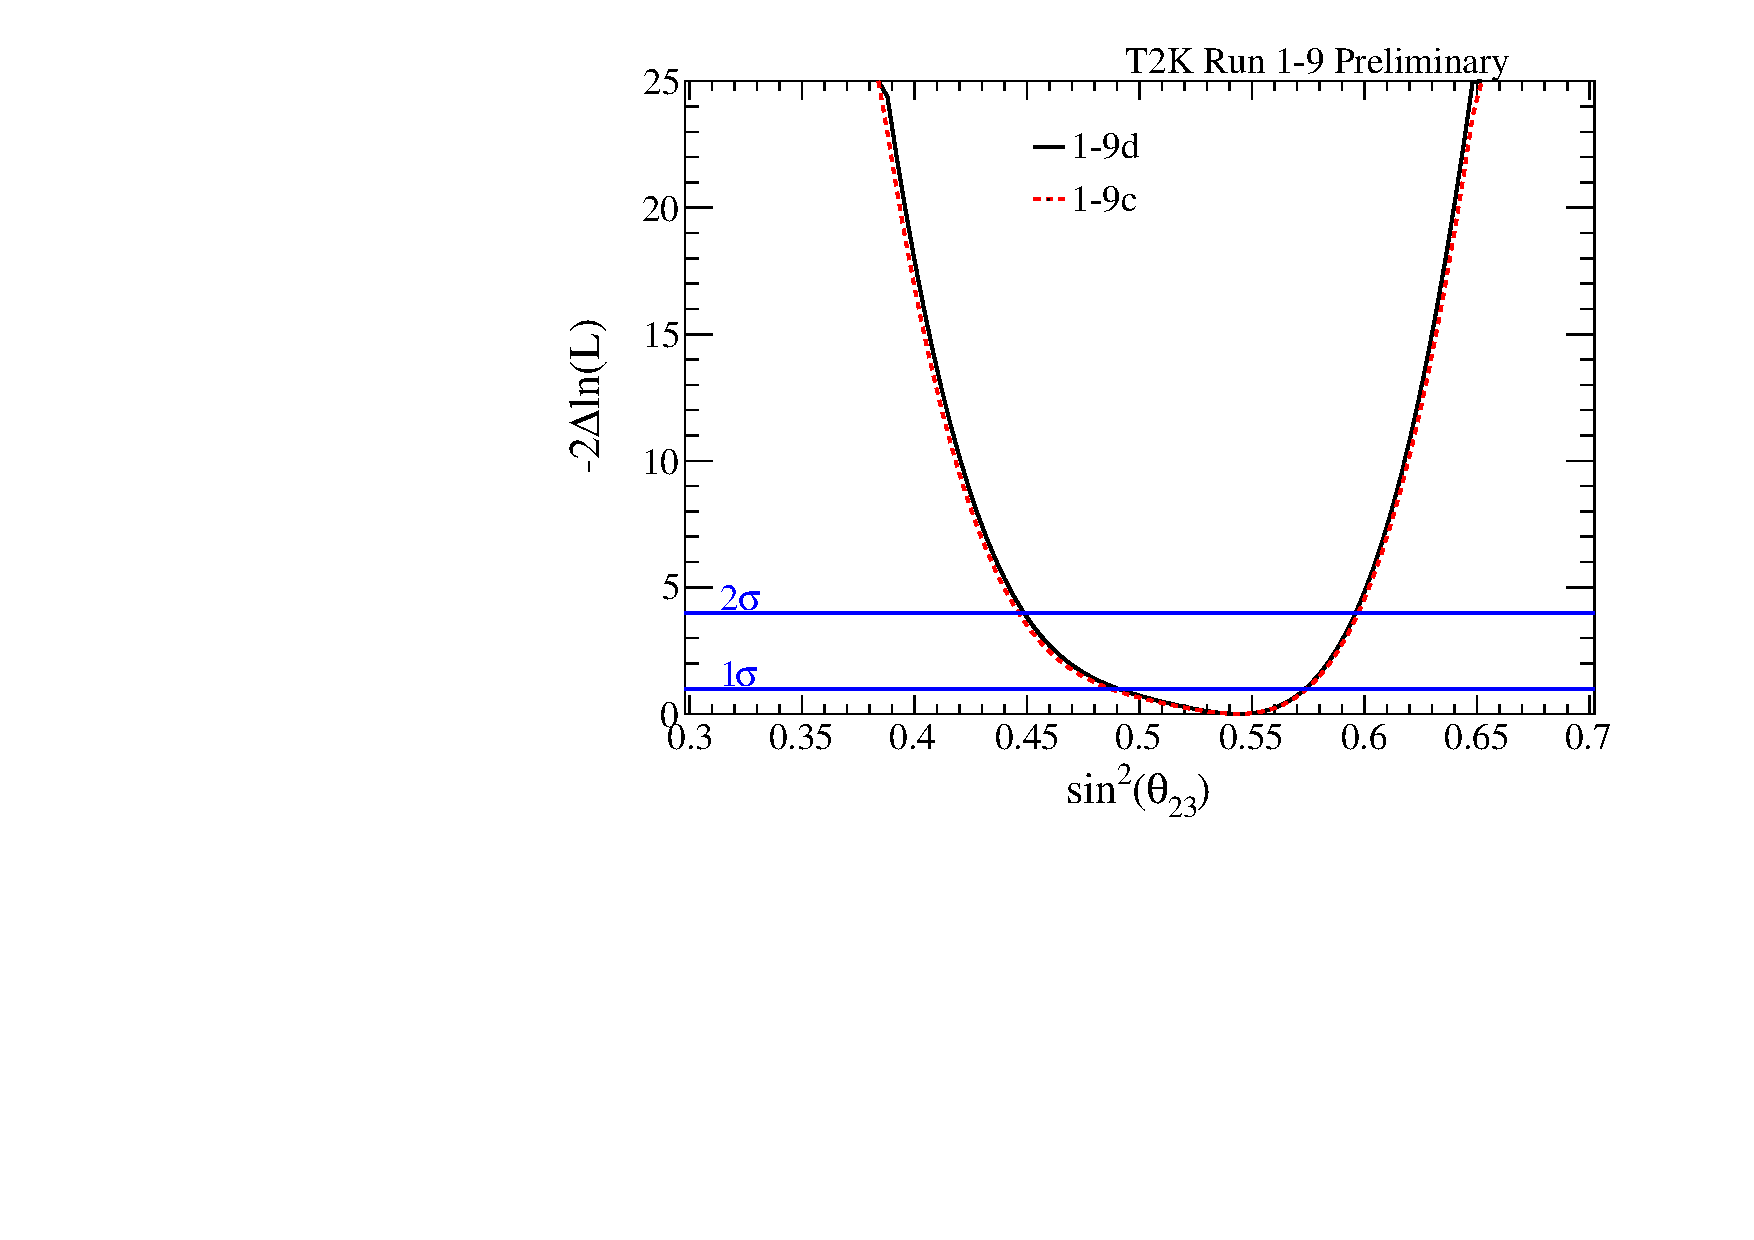
\includegraphics[width=0.9\textwidth]{images/sensitivity/comparison/theta23_wrc_inverted_1-9d_v_1-9c}
		\caption{\ssqthtwothree IH with reactor constraint}
	\end{subfigure}
	\begin{subfigure}[b]{0.49\textwidth}
		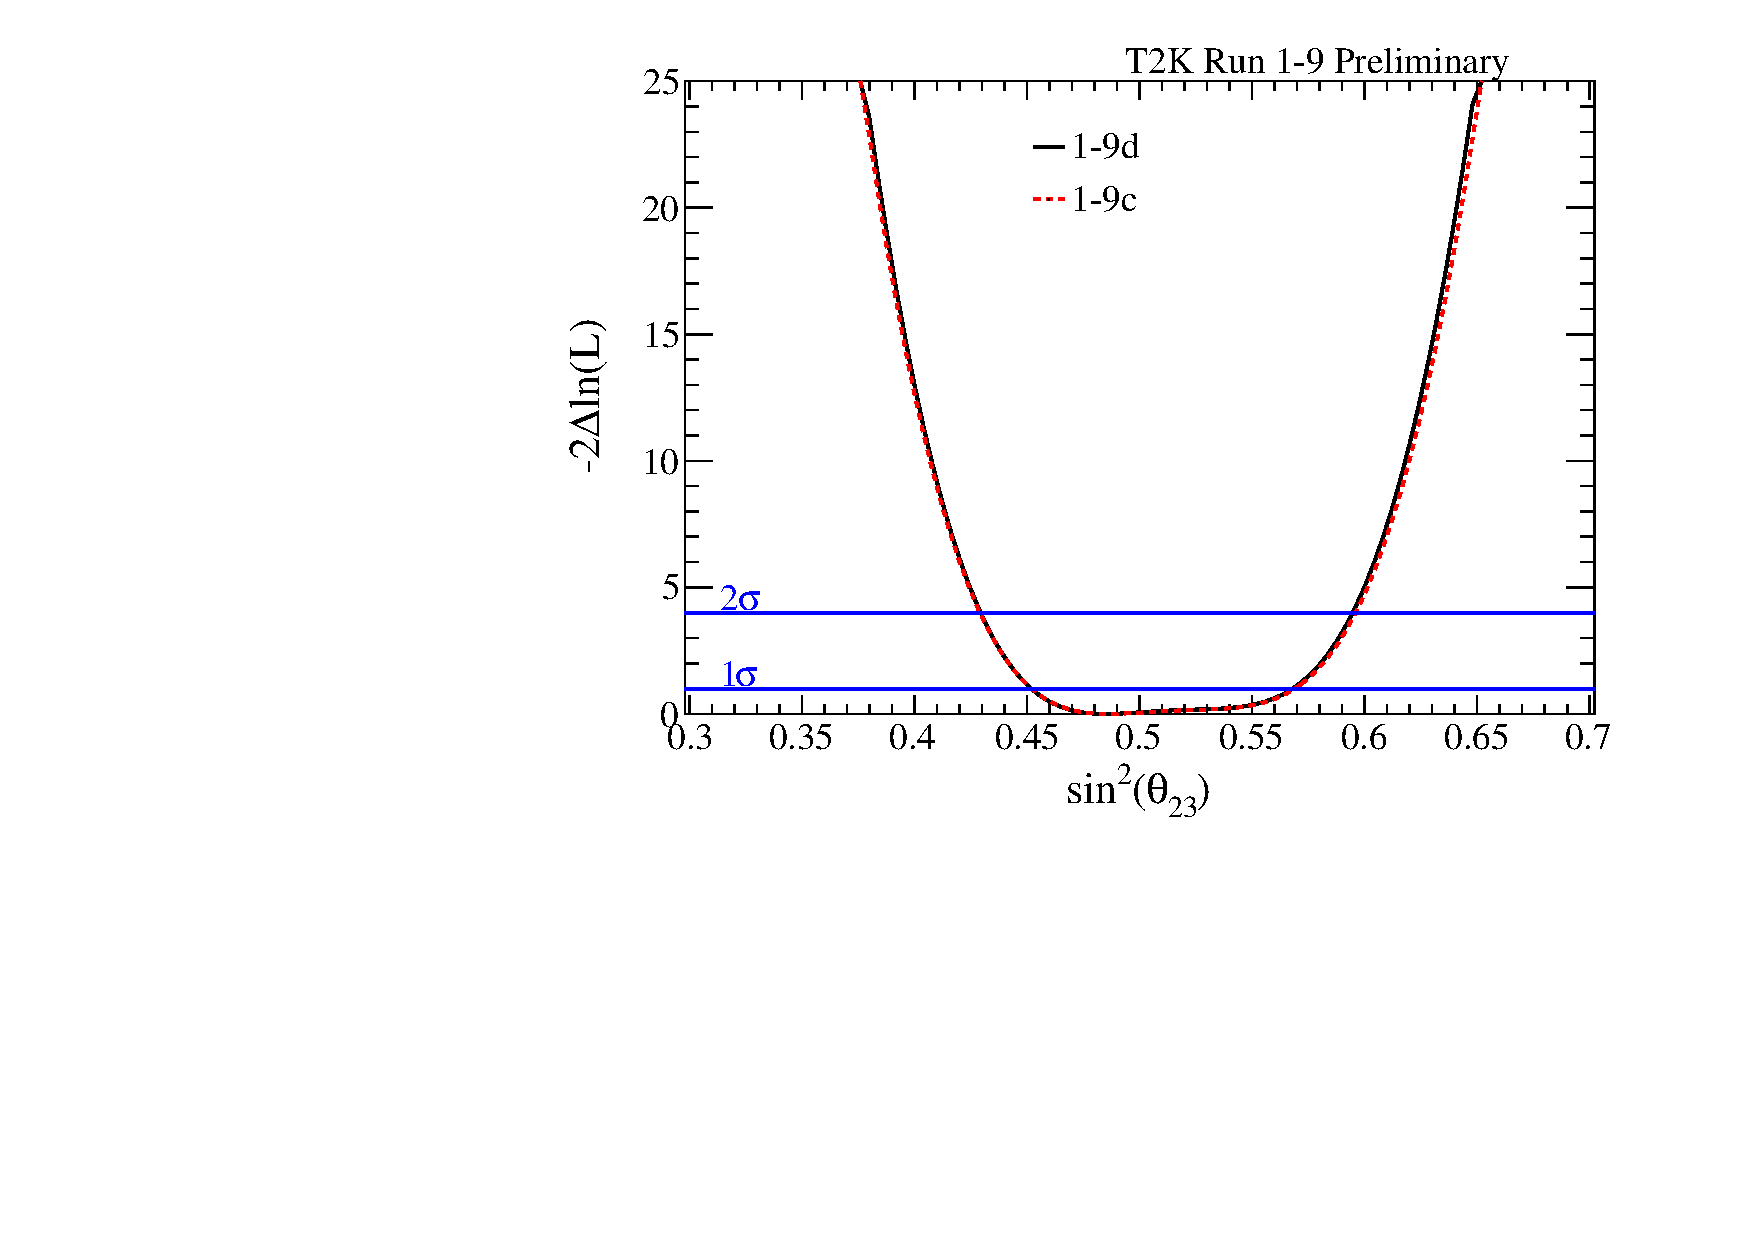
\includegraphics[width=0.9\textwidth]{images/sensitivity/comparison/theta23_worc_normal_1-9d_v_1-9c}
		\caption{\ssqthtwothree NH without reactor constraint}
	\end{subfigure}
	\begin{subfigure}[b]{0.49\textwidth}
		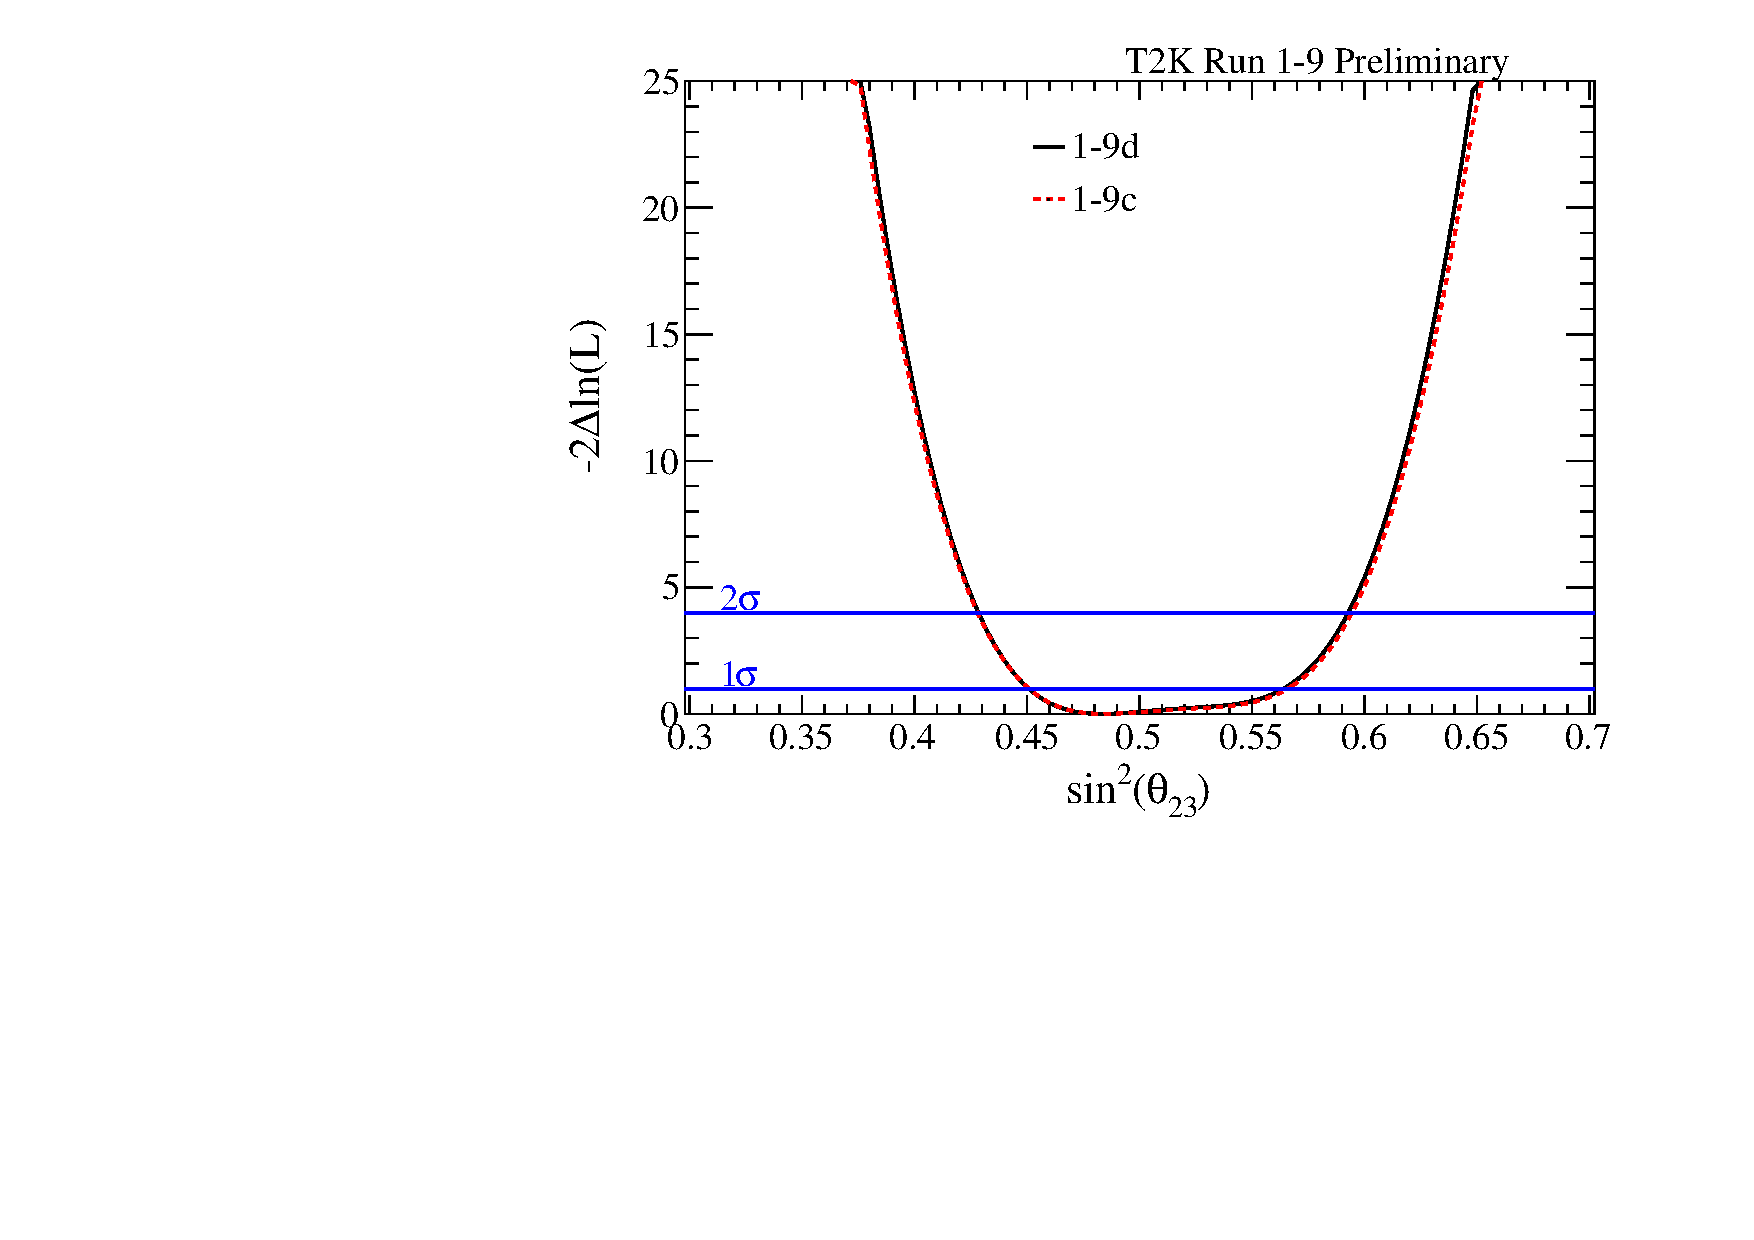
\includegraphics[width=0.9\textwidth]{images/sensitivity/comparison/theta23_worc_inverted_1-9d_v_1-9c}
		\caption{\ssqthtwothree IH without reactor constraint}
	\end{subfigure}
	\caption {
		The expected $\Delta\chi^2$ distribution as a function of \ssqthtwothree with and without reactor constraint. Normal and inverted hierarchy contours are independent. All 5 samples were used to produce these fits.
	}
	\label{fig:th23_asimov_compare}
\end{figure*}
\clearpage

\subsection{Results for \dmsq}

The result for \dmsq with reactor constraint and T2K only is shown in fig.~\ref{fig:dmsq_asimov_compare}.

\begin{figure*}[htb]
	\center
	\begin{subfigure}[b]{0.49\textwidth}
		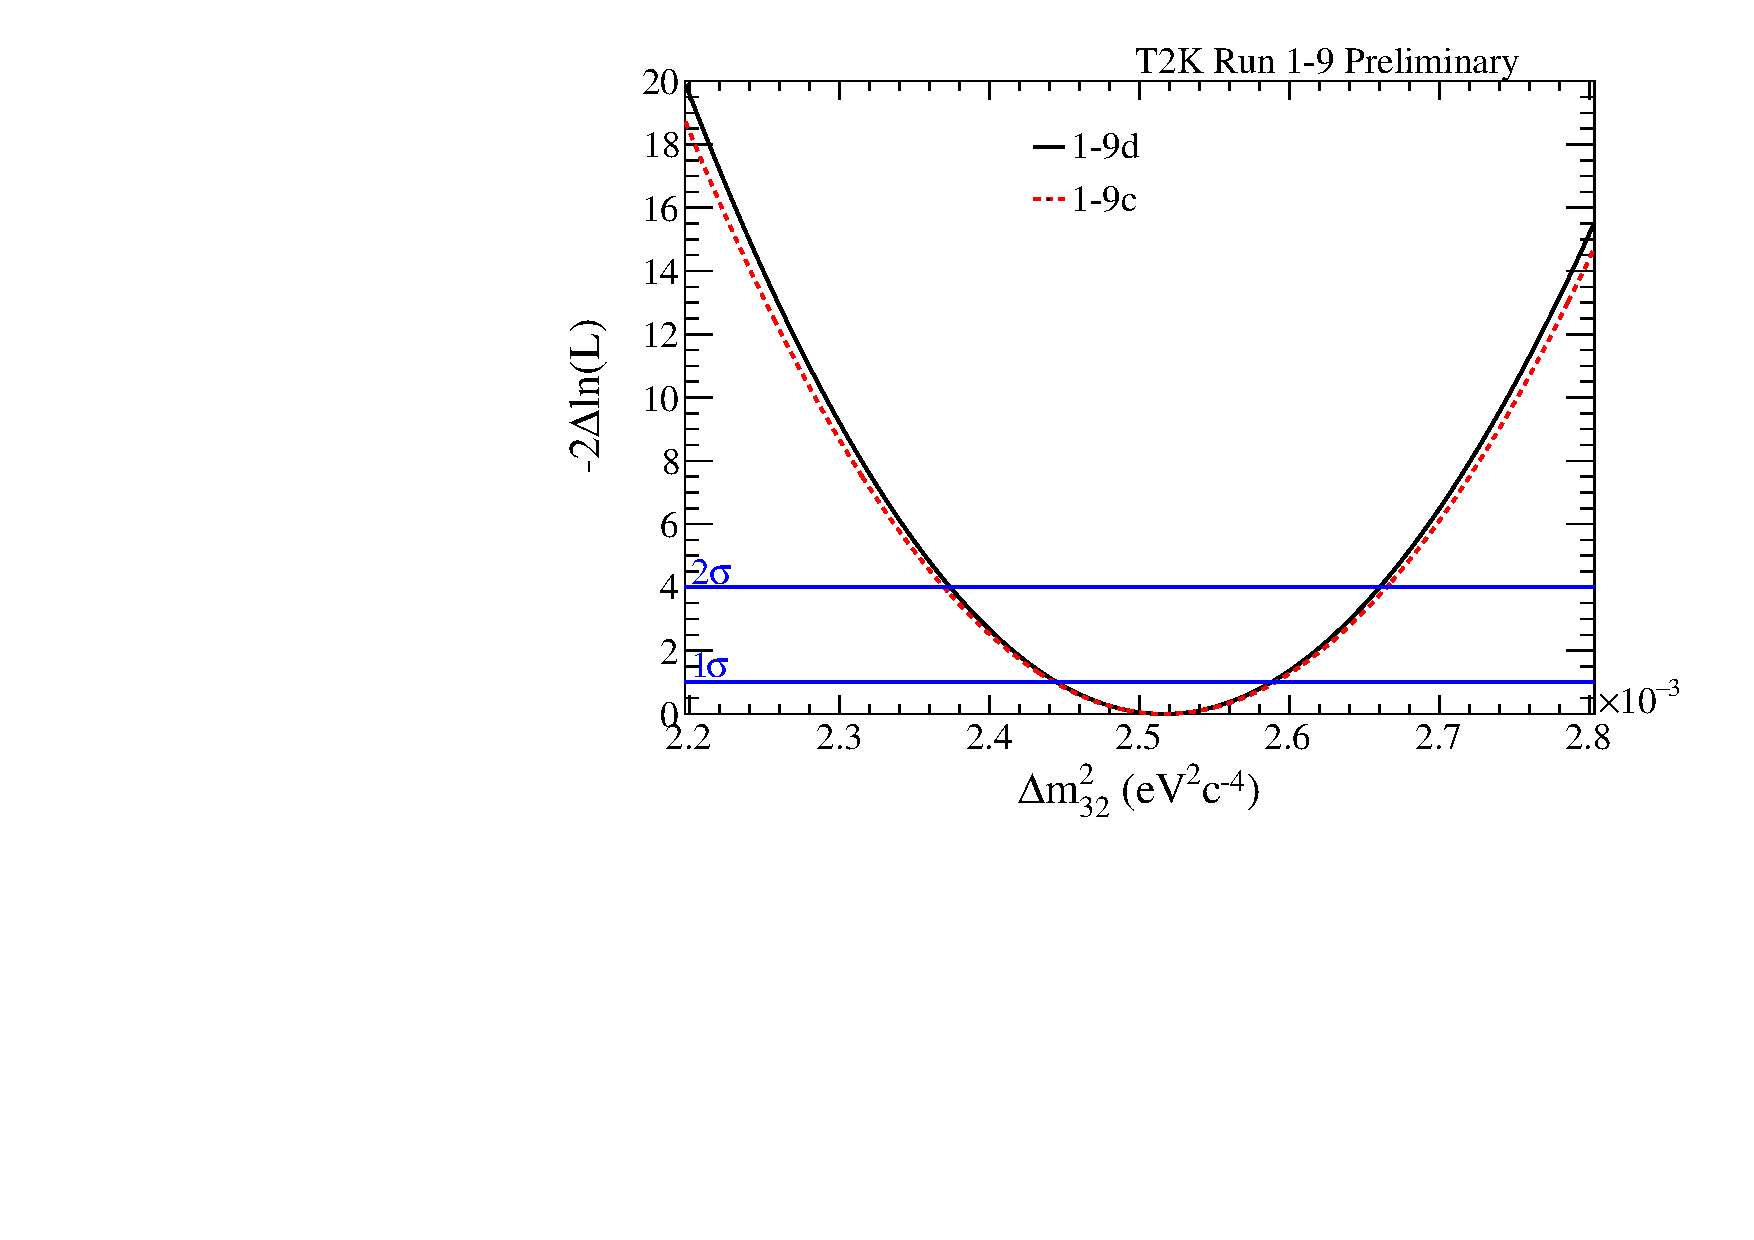
\includegraphics[width=0.9\textwidth]{images/sensitivity/comparison/dmsq_wrc_normal_1-9d_v_1-9c}
		\caption{\dmsq NH with reactor constraint}
	\end{subfigure}
	\begin{subfigure}[b]{0.49\textwidth}
		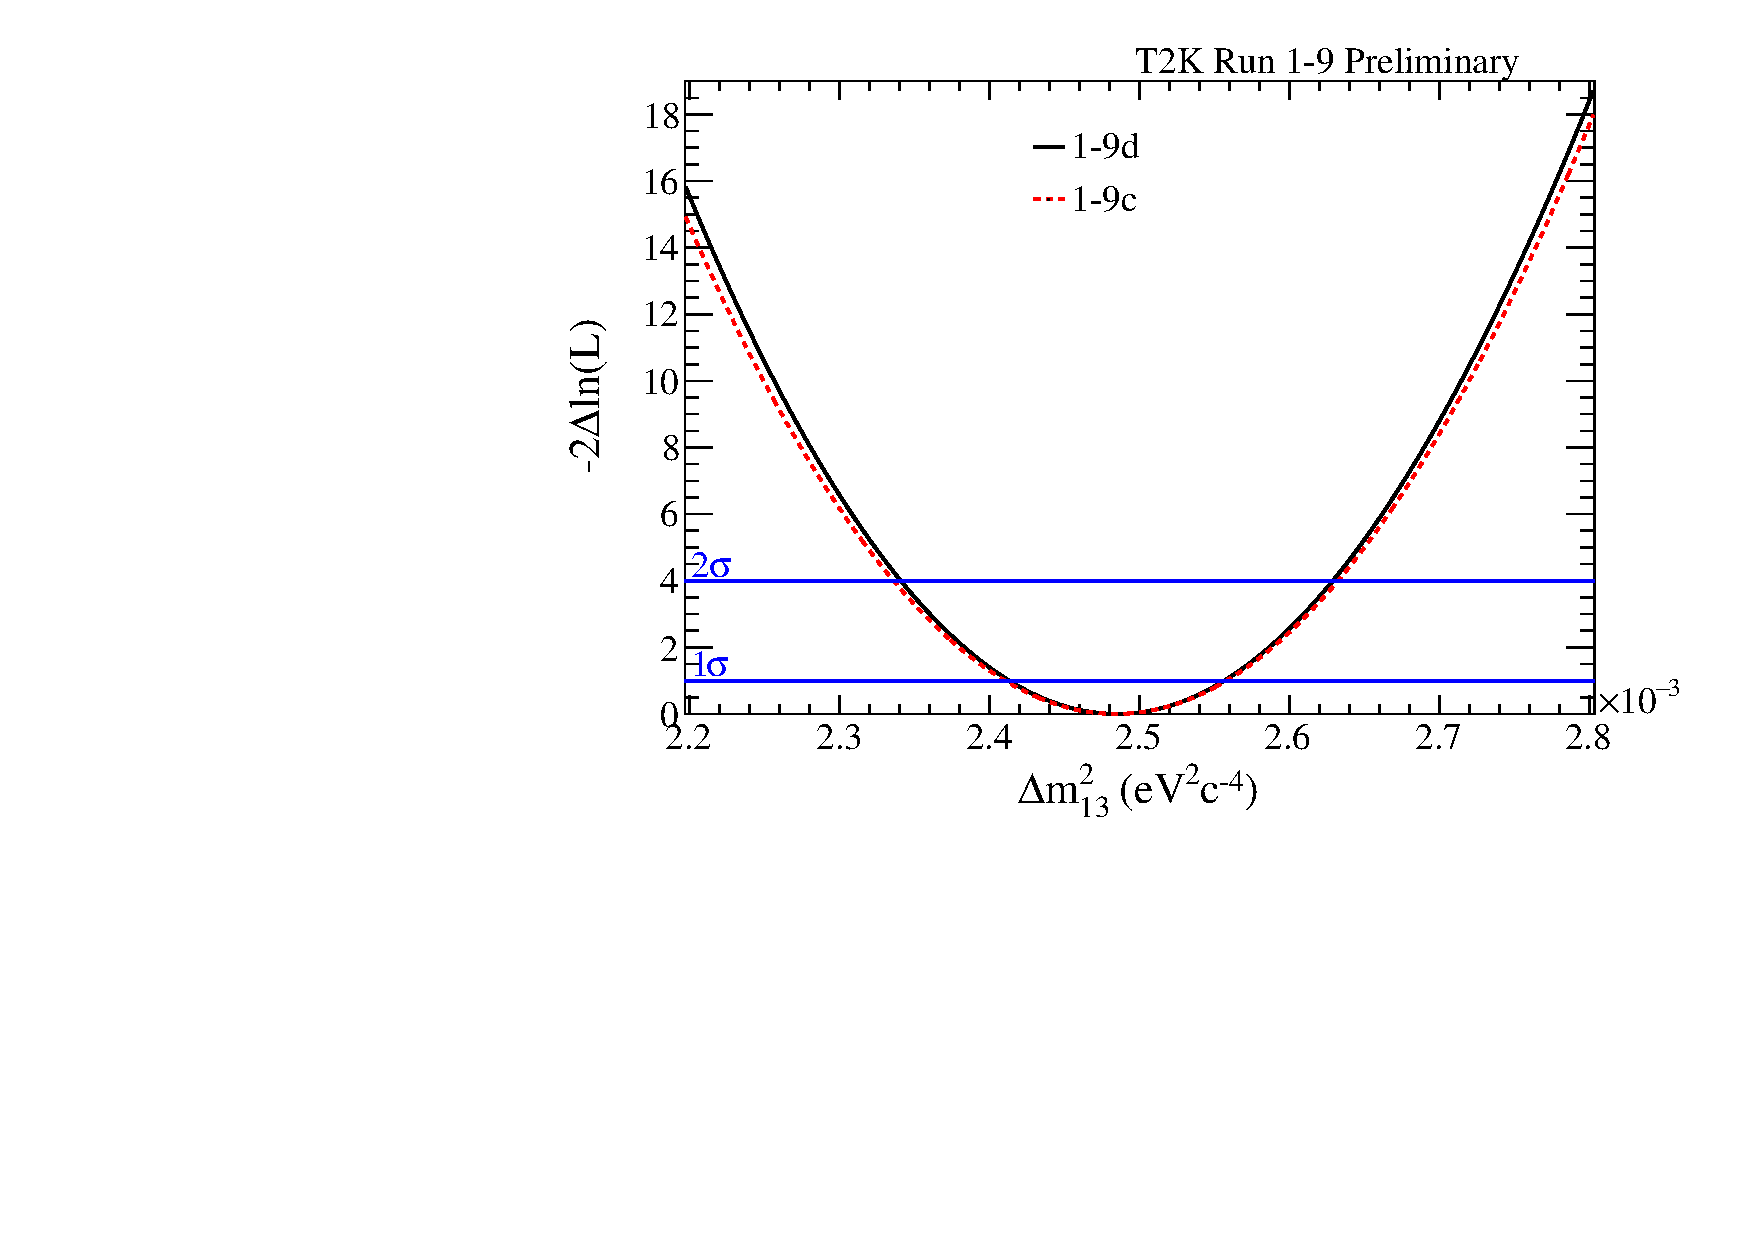
\includegraphics[width=0.9\textwidth]{images/sensitivity/comparison/dmsq_wrc_inverted_1-9d_v_1-9c}
		\caption{\dmsq IH with reactor constraint}
	\end{subfigure}
	\begin{subfigure}[b]{0.49\textwidth}
		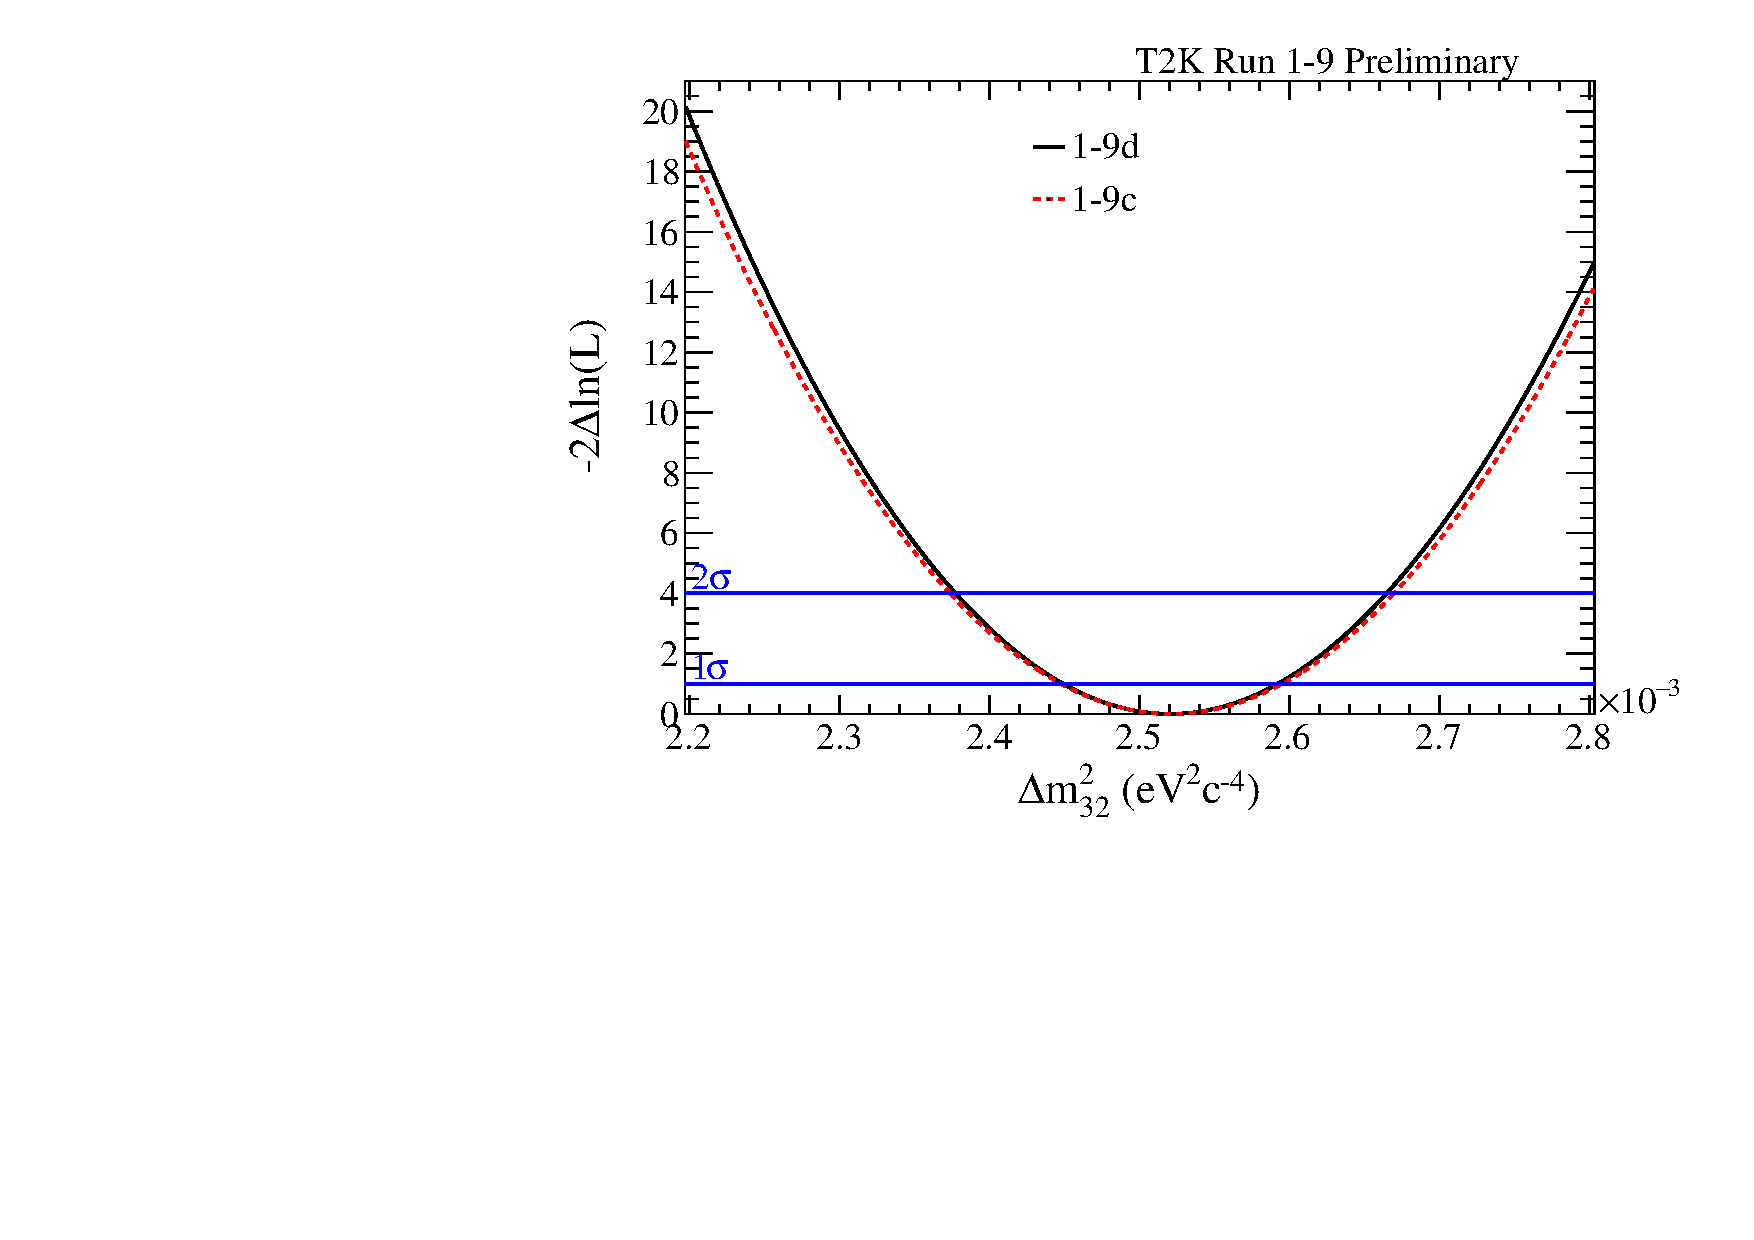
\includegraphics[width=0.9\textwidth]{images/sensitivity/comparison/dmsq_worc_normal_1-9d_v_1-9c}
		\caption{\dmsq NH without reactor constraint}
	\end{subfigure}
	\begin{subfigure}[b]{0.49\textwidth}
		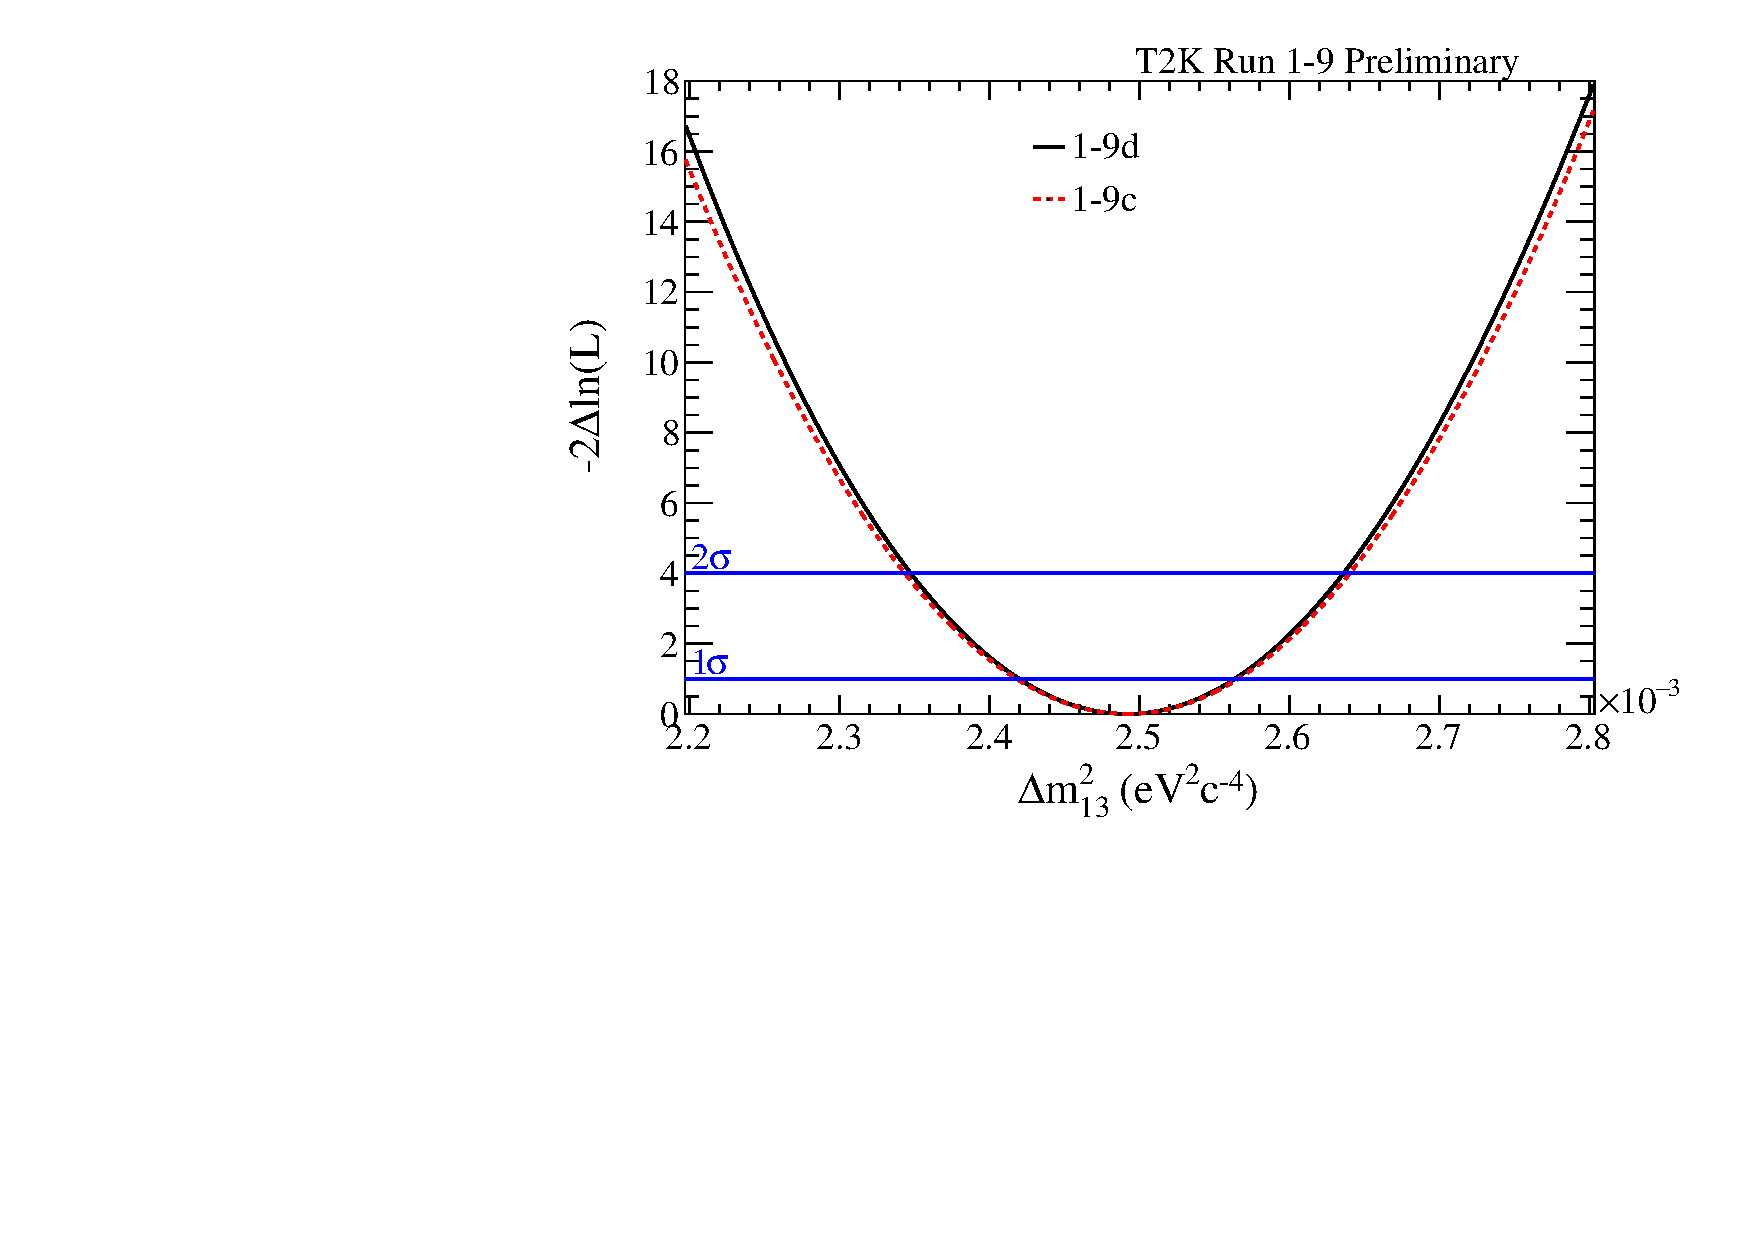
\includegraphics[width=0.9\textwidth]{images/sensitivity/comparison/dmsq_worc_inverted_1-9d_v_1-9c}
		\caption{\dmsq IH without reactor constraint}
	\end{subfigure}
	\caption {
		The expected $\Delta\chi^2$ distribution as a function of \dmsqtwothree with and without reactor constraint. Normal and inverted hierarchy contours are independent. All 5 samples were used to produce these fits.
	}
	\label{fig:dmsq_asimov_compare}
\end{figure*}

\clearpage